\documentclass[aspectratio=169]{beamer}
\usepackage{tikz}
\usepackage{graphicx}

\usecolortheme{whale}
\usetikzlibrary{er,positioning}  
\usetikzlibrary{decorations.pathreplacing}
\usetikzlibrary{arrows, decorations.markings}
\usetikzlibrary{shapes.geometric}
\usetikzlibrary{shapes.arrows}

\usepackage{listings}

\definecolor{blue1}{RGB}{126,126,206}
\definecolor{blue2}{RGB}{87,87,192}
\definecolor{blue3}{RGB}{51,51,178}
\definecolor{blue4}{RGB}{27,26,107}


\definecolor{cgreen}{RGB}{50,187,176}
\definecolor{cblue} {RGB} {53,140,214}
\lstdefinestyle{sharpc}{language=[Sharp]C, frame=lr, rulecolor=\color{blue!80!black}}

\usepackage{multicol}

\newcommand{\kword}[1]{{\color{cblue} \texttt{#1}}}
\newcommand{\tword}[1]{{\color{cgreen} \texttt{#1}}}

\setbeamertemplate{navigation symbols}{}

\setbeameroption{show notes on second screen=right}

\tikzstyle{every link} = []
\tikzstyle{link} = [>=triangle 60, draw, every link]

\definecolor{attr}{RGB}{10,153,2}

\title{Bases de Datos}
\subtitle{Dise\~no L\'ogico: Modelo relacional. Dise\~no Intuitivo}
\author[Garc\'ia L., Cardentey V. M., Ledesma A.]{
    Lic. Andy Ledesma Garc\'ia\\
    Lic. V\'ictor M. Cardentey Fundora\\ 
    Dra. C. Lucina Garc\'ia Hern\'andez
}
\institute[MATCOM-UH]{
    Departamento de Computaci\'on\\
    Facultad de Matem\'atica y Computaci\'on\\
    Universidad de La Habana\\[3mm]
    Licenciatura en Ciencia de Datos
}
\date[]{6 de febrero de 2024}


\begin{document}
    \maketitle
    \begin{frame}{¿Hasta d\'onde hemos llegado?}
    \centering
    \resizebox{14cm}{7.5cm}{
    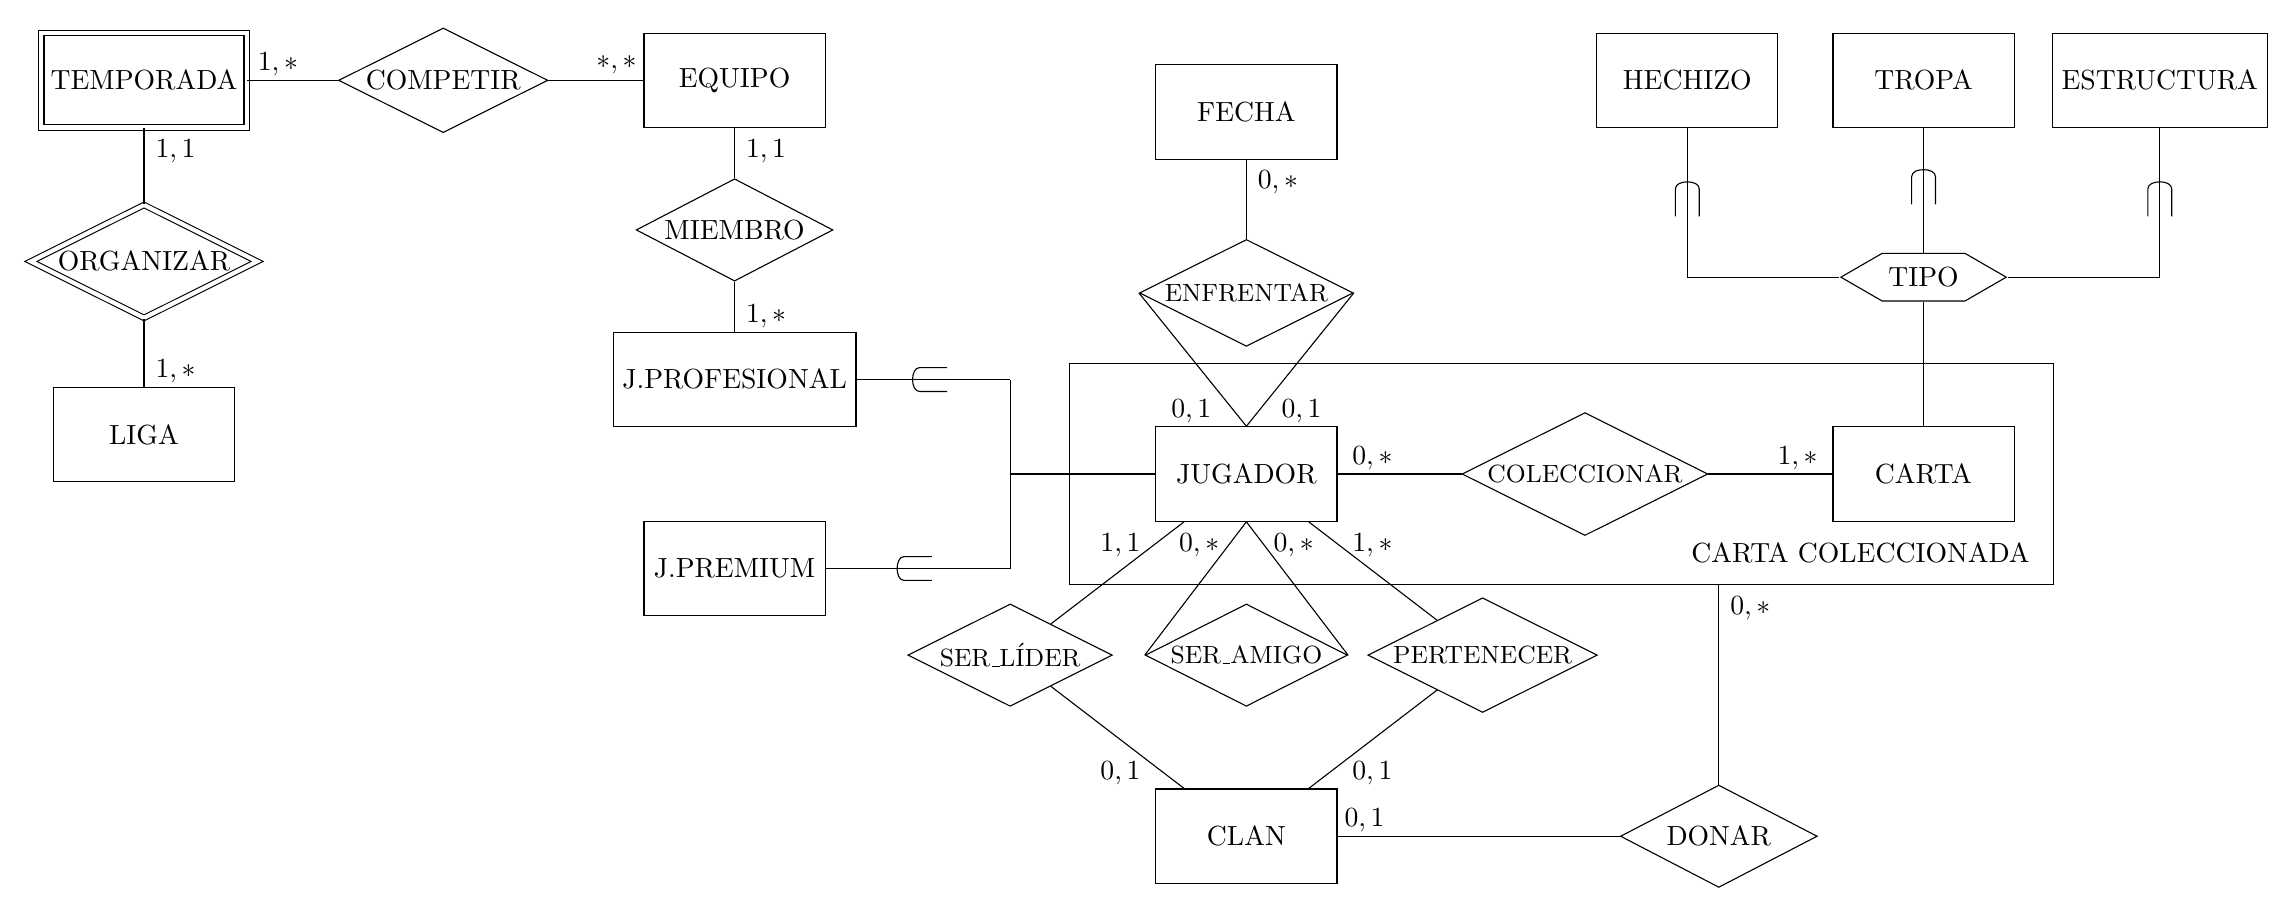
\begin{tikzpicture}
        \tikzstyle{every entity} = [minimum width=2.3cm, minimum height=1.2cm]
        \tikzstyle{every relationship} = [minimum width=2.5cm, minimum height=1.3cm]
        \tikzset{link/.append style={
            postaction={decorate},
            decoration={
                markings,
                mark= at position 0.5 with {
                    \draw (0.5em,1ex) -- (-0.5em,1ex) to[bend right=90] (-0.5em,-1ex) -- (0.5em,-1ex);
                }
            }
        }}
        \node[entity] (jugador) at (0,0) {JUGADOR};
        \node[entity] (fecha) at (0,4.6) {FECHA};
        \node[entity] (clan) at (0,-4.6) {CLAN};
        \node[entity] (carta) at (8.6,0) {CARTA};

        

        \node[entity] (tropa) at (8.6, 5) {TROPA};
        \node[entity] (estructura) at (11.6,5) {ESTRUCTURA};
        \node[entity] (hechizo) at (5.6,5) {HECHIZO};

        \node[regular polygon, draw, regular polygon sides=6, minimum width=7mm, xscale=3, label=center:TIPO] (tipo) at (8.6,2.5) {};
        \draw (carta.north) -- (tipo.south);
        \draw (tipo.west) -- (5.6,2.5);
        \draw (tipo.east) -- (11.6,2.5);
        \draw[link] (tropa.south) -- (tipo.north);
        \draw[link] (hechizo.south) -- (5.6,2.5);
        \draw[link] (estructura.south) -- (11.6,2.5);


        \node[relationship,aspect=2] (pertenecer) at (3,-2.3) {\small PERTENECER}
            edge(jugador) edge(clan);
        \node at (1.6,-0.9) {$1,\ast$};
        \node at (1.6,-3.8) {$0,1$};

        \node at (1.5,-4.4) {$0,1$};
        \node at (6.4,-1.7) {$0,\ast$};

        \node at (0.6,-0.9) {$0,\ast$};
        \node at (-0.6,-0.9) {$0,\ast$};

        \node[relationship,aspect=2] (coleccionar) at (4.3,0) {\small COLECCIONAR}
            edge(carta) edge(jugador);
        \node at (1.6,0.2) {$0,\ast$};
        \node at (7.0,0.2) {$1,\ast$};

        \node[relationship,aspect=2] (enfrentar) at (0,2.3) {\small ENFRENTAR}
            edge(fecha);
        \draw (enfrentar.west) -- (jugador.north);
        \draw (enfrentar.east) -- (jugador.north);
        \node at (0.7,0.8) {$0,1$};
        \node at (-0.7,0.8) {$0,1$};
        \node at (0.4,3.7) {$0,\ast$};

        \node[relationship,aspect=2] (seramigo) at (0, -2.3) {\small SER\_AMIGO};
        \draw (seramigo.east) -- (jugador.south);
        \draw (seramigo.west) -- (jugador.south);

        \node[relationship,aspect=2] (serlider) at (-3,-2.3) {\small SER\_L\'IDER}
            edge(jugador) edge(clan);
        \node at (-1.6,-3.8) {$0,1$};
        \node at (-1.6,-0.9) {$1,1$};

        \node[rectangle, draw, minimum width=12.5cm, minimum height=2.8cm] at (4,0) {};
        \node at (7.8,-1) {CARTA COLECCIONADA};

        \node[relationship, aspect=2] (donar) at (6,-4.6) {DONAR} edge(clan);
        \draw (6,-1.4) -- (donar.north);

        
        \draw (-3,0) -- (jugador.west);
        
        \node[entity] (premium) at (-6.5,-1.2) {J.PREMIUM};
        \node[entity] (profesional) at (-6.5,1.2) {J.PROFESIONAL};
        \draw (-3,0) -- (-3,-1.2);
        \draw (-3,0) -- (-3,1.2);
        \draw[link] (premium.east) -- (-3,-1.2);
        \draw[link] (profesional.east) -- (-3,1.2);


        \node[entity] (equipo) at (-6.5,5) {EQUIPO};
        \node at (-6.1,4.1) {$1,1$};
        \node at (-6.1,2) {$1,\ast$};

        \node[relationship,aspect=2] (miembro) at (-6.5,3.1) {MIEMBRO} edge(profesional) edge(equipo); 

        \node[entity,double distance=1.5pt] (temporada) at (-14, 5) {TEMPORADA};


        \node[entity] (liga) at (-14,0.5) {LIGA};
        \node[relationship,aspect=2,double distance=1.5pt] (organizar) at (-14,2.7) {ORGANIZAR} edge(temporada) edge(liga);

        \node[relationship,aspect=2] (compet) at (-10.2,5) {COMPETIR} edge(temporada) edge(equipo);
        
        \node at (-8,5.2) {$\ast,\ast$};
        \node at (-12.3,5.2) {$1,\ast$};

        \node at (-13.6,4.1) {$1,1$};
        \node at (-13.6,1.3) {$1,\ast$};
       
        



        
    \end{tikzpicture}
    }
\end{frame}

\begin{frame}{¿De d\'onde partimos?}
    \centering
    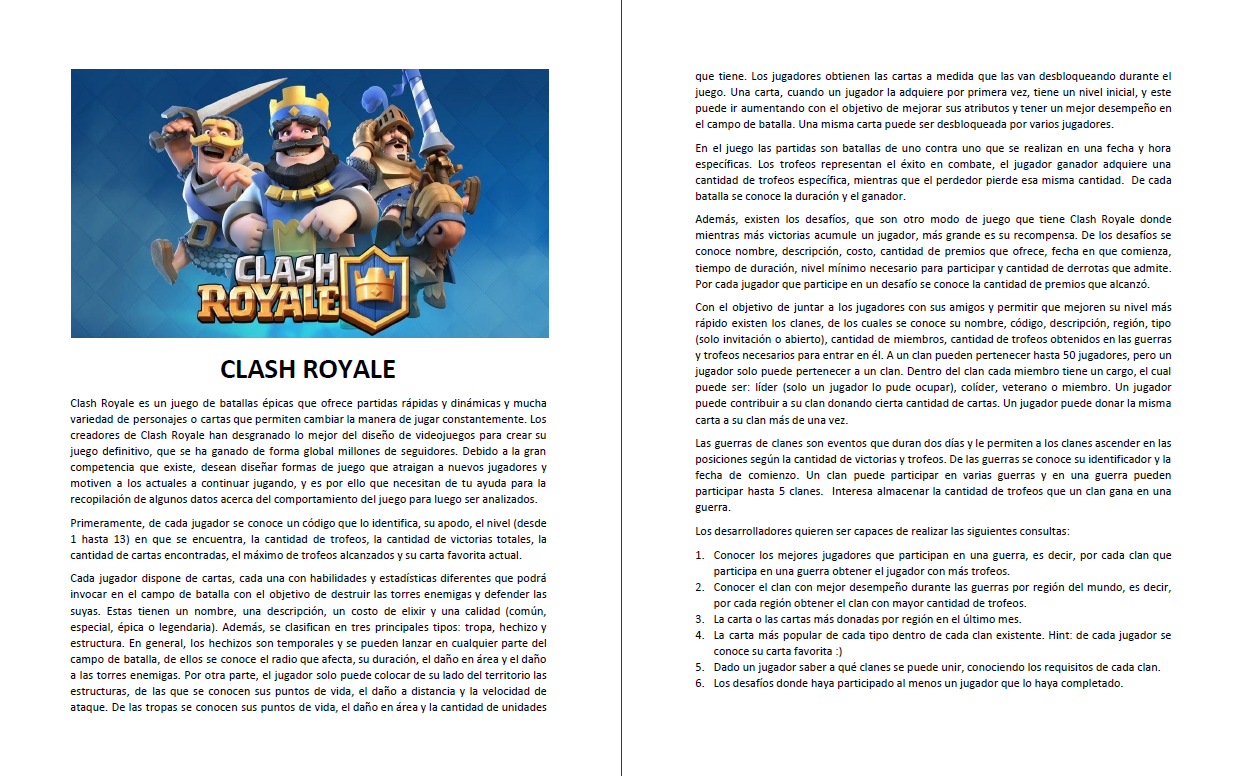
\includegraphics[width=0.8\linewidth, height=0.8\textheight]{img/specs.png}
\end{frame}

\begin{frame}{¿C\'omo obtener una especificaci\'on?}
    \begin{block}{An\'alisis de requerimientos}
        \begin{itemize}
            \item Descripciones en lenguaje natural
            \item Encuestas
            \item Observaci\'on directa 
            \item Formatos de registros
            \item Esquemas de datos
        \end{itemize}
    \end{block}
\end{frame}
    \begin{frame}
    \frametitle{Objetivos de la clase de hoy}

    \begin{itemize}[<+->]
        \item Reconocer la vigencia y las limitaciones de las bases de datos relacionales. 
        \item Brindar una breve panorámica de las motivaciones y los fundamentos de las bases de datos NoSQL.
        \item Mencionar los principales retos que se presentan al migrar de un sistema de gestión de bases de datos relacionales a uno NoSQL.
    \end{itemize}
\end{frame}
    \begin{frame}{Representaci\'on tabular}
    \begin{columns}[T]
        \begin{column}{0.48\linewidth}
            \vspace{25mm}

            \resizebox{\linewidth}{!}{
                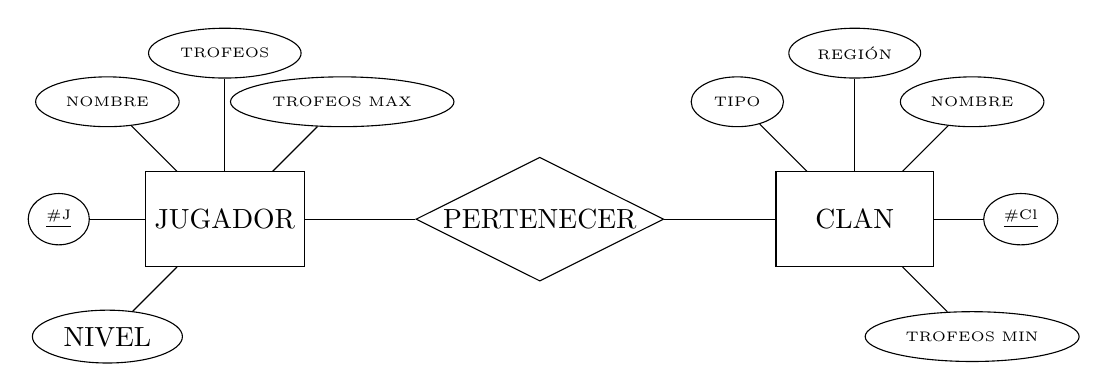
\begin{tikzpicture}[node distance=6em]
                    \tikzstyle{every entity} = [minimum width=2cm, minimum height=1.2cm]
                    \node[entity] (jugador) {JUGADOR}
                        [sibling distance=3cm]
                        child {node[attribute] [above right of=jugador] {\tiny TROFEOS MAX}}
                        child {node[attribute] [above of=jugador] {\tiny TROFEOS}}
                        child {node[attribute] [above left of=jugador] {\tiny NOMBRE}}
                        child {node[attribute] [left of=jugador] {\underline{\tiny \#J}}}
                        child {node[attribute] [below left of=jugador] {NIVEL}}
                        ;
                  
                    \node[entity] (clan) at (8,0) {CLAN}
                    [sibling distance=3cm]
                    child {node[attribute] [right of=clan] {\underline{\tiny \#Cl}}}
                    child {node[attribute] [above of=clan] {\tiny REGI\'ON}}
                    child {node[attribute] [above left of=clan] {\tiny TIPO}}
                    child {node[attribute] [above right of=clan] {\tiny NOMBRE}}
                    child {node[attribute] [below right of=clan] {\tiny TROFEOS MIN}};

                    \node[relationship,aspect=2] (pertenecer) at (4,0) {PERTENECER}
                    edge(jugador) edge(clan);
                \end{tikzpicture}
            }
        \end{column}

        \begin{column}{0.48\linewidth}

            \begin{center}

                \vspace{-5mm}

                \tiny{JUGADOR}
                \vspace{2mm}

                \begin{tiny}
                    
                    \begin{tabular}{|c|c|c|c|c|}
                        \hline
                        \underline{\#J} & Nombre & Nivel& Trofeos & TrofeosMax\\
                        \hline
                        1 & Juan & 13 & 7500 & 7560\\
                        \hline
                        2 & Pedro &  11 & 7000 & 7200 \\
                        \hline
                        3 & Mar\'ia & 12  & 7050 & 7400\\
                        \hline
                        $\vdots$ & $\vdots$ & $\vdots$ & $\vdots$ & $\vdots$\\
                        \hline
                        
                    \end{tabular}
                \end{tiny}
                
                \vspace{3mm}

                \tiny{CLAN}
                \vspace{2mm}

                \begin{tiny}
                    \begin{tabular}{|c|c|c|c|c|}
                        \hline
                        \underline{\#C} & Nombre & Regi\'on & Tipo & TrofeosMin\\
                        \hline
                        1 & River Plate 2. & MEX & Cerrado & 7000 \\
                        \hline
                        2 & TheWarriors & GER & Invitaci\'on & 7300\\
                        \hline
                        3 & WestRoyale &  ESP & Cerrado & 6300\\
                        \hline
                        $\vdots$ & $\vdots$ & $\vdots$ & $\vdots$ & $\vdots$\\
                        \hline
                        
                    \end{tabular}
                \end{tiny}
                
                \vspace{3mm}

                \tiny{PERTENECER}
                \vspace{2mm}

                \begin{tiny}
                    \begin{tabular}{|c|c|}
                        \hline
                        \underline{\#J} & \underline{\#C}\\
                        \hline
                        1 & 2  \\
                        \hline
                        2 & 3\\
                        \hline
                        3 & 1\\
                        \hline
                        $\vdots$ & $\vdots$\\
                        \hline
                    \end{tabular}
                \end{tiny}
                
            \end{center}
        \end{column}
        
    \end{columns}

    \note{@NOTE existen diversas estructuras de datos para representar un MERX l\'ogicamente: \'arboles, grafos... pero las tablas ofrecen muchas facilidades como la f\'acil comprensi\'on que de ellas puede hacer el interlocutor... Necesitamos una base matem\'atica-computacional que sostenga esta representaci\'on, que le d\'e formalidad, consistencia y confiabilidad.}
\end{frame}

\begin{frame}{¿C\'omo podemos describir un MERX?}

    \begin{block}<2->{Modelo matem\'atico de datos}
        Un modelo matem\'atico de datos es una definici\'on l\'ogica,
        abstracta y auto-contenida de: \begin{itemize}
            \item<3-> \textbf{Estructuras de datos}: utilizadas para la representaci\'on de los datos
            y sus interrelaciones.
            \item<4-> \textbf{Restricciones de integridad}: utilizadas para mantener un estado consistente
            de la base de datos durante la ejecuci\'on de operaciones que modifican la base de datos.
            \item<5-> \textbf{Operaciones}: utilizadas para manipular los datos.
        \end{itemize}
        \onslide<6->{que integradas constituyen una m\'aquina abstracta con la que los usuarios interact\'uan.}
    \end{block}
    
\end{frame}


\begin{frame}{La implementaci\'on no es una descripci\'on}
    \begin{block}{Implementaci\'on de un modelo matem\'atico de datos}
        Es una realizaci\'on f\'isica
        en una m\'aquina real de los componentes
        de la m\'aquina abstracta que constituye el modelo.\\[5mm]
    \end{block}
\end{frame}


    \begin{frame}{Todo es acerca de la conveniencia}
    \centering
    \begin{tikzpicture}
        \node at (1.4,7) {\tiny \bf {Usuario de SGBD}} ;
        \node[inner sep=0pt] at (1.4,5.8) {
            
\includegraphics[width=1.8cm]{img/hface.png}
        };

        \node at (1.4,4.3) {\tiny \bf {Desarrollador de SGBD}} ;
        \node[inner sep=0pt] at (1.4,3.2) {
            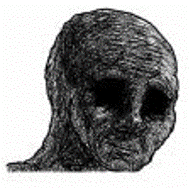
\includegraphics[width=1.8cm]{img/sface.png}
        };

        \draw[-,thick] (0.3, 4.6) -- (7,4.5);
        \draw[-,thick] (2.7, 2) -- (2.7,7.4);

        \onslide<1>{
        \node at (5,5.8) {Lenguaje declarativo};
        \node at (5,4.3) {Estructuras de datos};%\\Algoritmos\\Optimizaci\'on\\Compilaci\'on\\Gesti\'on de ficheros};
        \node at (5,3.8) {Algoritmos};%\\Algoritmos\\Optimizaci\'on\\Compilaci\'on\\Gesti\'on de ficheros};
        \node at (5,3.3) {Optimizaci\'on};%\\Algoritmos\\Optimizaci\'on\\Compilaci\'on\\Gesti\'on de ficheros};
        \node at (5,2.8) {Compilaci\'on};%\\Algoritmos\\Optimizaci\'on\\Compilaci\'on\\Gesti\'on de ficheros};
        \node at (5,2.3) {Gesti\'on de ficheros};%\\Algoritmos\\Optimizaci\'on\\Compilaci\'on\\Gesti\'on de ficheros};
        }

        \onslide<2>{
            \node at (5.3,5.8) {Modelo matem\'atico de datos};
            \node at (5,3) {Implementaci\'on};%\\Algoritmos\\Optimizaci\'on\\Compilaci\'on\\Gesti\'on de ficheros};

        }
    \end{tikzpicture}


\end{frame}

{
\setbeamertemplate{background} 
{
    
\includegraphics[width=\paperwidth,height=\paperheight]{img/prerelational.jpg}
}
\begin{frame}
\end{frame}
}

\begin{frame}{Enfoques pre-relacionales}
    \vspace{5mm}
    \begin{overlayarea}{\linewidth}{\textheight}
        
        \begin{block}<1->{Importancia}
            \begin{itemize}
                \item Fueron las primeras soluciones computacionales capaces de almacenar y consultar grandes conjuntos de datos.
                \item Se desarrollaron productos comerciales de larga vida basados en estos sistemas.
            \end{itemize}
            
        \end{block}
    
        \begin{block}<2->{Problemas}
            \begin{itemize}
                \only<2>{
                \item Los modelos de datos se consideran como abstracciones de
                las estructuras de almacenamiento subyacentes en el nivel
                físico y sus operadores asociados.}
                \item<3-> El modelo depend\'ia de la implementaci\'on.
                \only<4>{
                \item Los datos se representan por colecciones de registros
                (\textit{records}) y las interrelaciones entre los datos se representan
                mediante enlaces (\textit{links}).}
                \item<5-> Eran muy complicados de utilizar.
                \item<6-> Los usuarios son programadores que se deben encargar, incluso, de la optimizaci\'on.
    
            \end{itemize}
        \end{block}
    \end{overlayarea}
\end{frame}


\begin{frame}{Modelos jer\'arquico y reticular}
    \begin{columns}
        \begin{column}[t]{.5\textwidth}
            \begin{block}{Modelo jer\'arquico}
                \begin{itemize}[<+->]
                \item Las interrelaciones se representan como jerarqu\'ias.
                \item Ning\'un hijo puede existir sin su padre.
                \item Se recorre un \'arbol para: \textcolor<7>{red}{insertar}, \textcolor<7>{red}{actualizar}, \textcolor<7>{red}{eliminar} y \textcolor<7>{red}{buscar}.
                \end{itemize}
            \end{block}
        \end{column}

        \begin{column}[t]{.5\textwidth}
            \begin{block}<4->{Modelo reticular}
                \begin{itemize}[<+->]
                \item Las interrelaciones se representan a trav\'es de un grafo orientado.
                \item No tiene restricciones de integridad.
                \item Se recorre un grafo para: \textcolor<7>{red}{insertar}, \textcolor<7>{red}{actualizar}, \textcolor<7>{red}{eliminar} y \textcolor<7>{red}{buscar}.
                \end{itemize}
            \end{block}
        \end{column}
    \end{columns}
\end{frame}

\begin{frame}{Una imagen vale m\'as que mis palabras}
    \begin{columns}
        \column{0.5\textwidth}
        \centering
        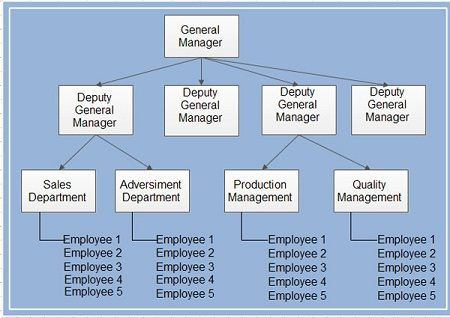
\includegraphics[width=\textwidth]{img/Hierarchical-Model.jpg}

        \column{0.5\textwidth}
            \centering
            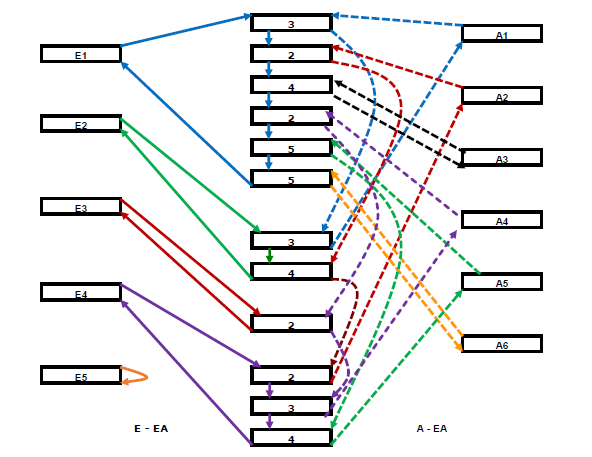
\includegraphics[width=\textwidth, height=0.8\textheight]{img/reticular.png}
    \end{columns}
\end{frame}





    \begin{frame}{Por fin...}
    \begin{block}{Propuesta de E. F. Codd (1970)}
        \begin{itemize}
            \item Relacionar los datos mediante v\'inculos
            naturales, l\'ogicos, inherentes a los datos y al fen\'omeno y no
            a su representaci\'on computacional. 
            \item Lograr un modelo simple en el que tanto los datos
            como los v\'inculos que se establecen entre ellos se representen
            mediante tablas.
        \end{itemize}
        
    \end{block}
\end{frame}


\begin{frame}{¿Est\'an listos chicos?}
    
\includegraphics[width=\linewidth, height=0.85\textheight]{img/relational_model.jpg}
\end{frame}
    \begin{frame}{Modelo relacional}
    \centering
    \Huge \textcolor{blue3}{Estructura de datos}

    \note{@NOTE cu\'al es el modelo matem\'atico de datos para el modelo relacional}
\end{frame}

\begin{frame}{¿C\'omo describir una tabla?}
    \begin{LARGE}
        
        ¿Qu\'e conceptos matem\'aticos pudiesen modelar una tabla?
    \end{LARGE}
    


    \begin{center}
        JUGADOR
        \vspace{2mm}

        \begin{tabular}{|c|c|c|c|c|}
            \hline
            \underline{\#J} & Nombre & Nivel& Trofeos & TrofeosMax\\
            \hline
            1 & Juan & 13 & 7500 & 7560\\
            \hline
            2 & Pedro &  11 & 7000 & 7200 \\
            \hline
            3 & Mar\'ia & 12  & 7050 & 7400\\
            \hline
            $\vdots$ & $\vdots$ & $\vdots$ & $\vdots$ & $\vdots$\\
            \hline
            
        \end{tabular}
    \end{center}
   
\end{frame}

\begin{frame}{¿Nos servir\'a alguna estructura matem\'atica que ya conocemos?}
    \centering
    \begin{LARGE}
        
        ¿Podemos utilizar una matriz?
    \end{LARGE}
    
    \vspace{5mm}

    \[
  A_{m\times n} =
  \left[ {\begin{array}{cccc}
    a_{11} & a_{12} & \cdots & a_{1n}\\
    a_{21} & a_{22} & \cdots & a_{2n}\\
    \vdots & \vdots & \ddots & \vdots\\
    a_{m1} & a_{m2} & \cdots & a_{mn}\\
  \end{array} } \right]
\]

\vspace{5mm}

\onslide<2>{
\centering
    \begin{LARGE}
       \textcolor{red}{No. Las matrices se definen sobre un \'unico dominio}
    \end{LARGE}
}



\end{frame}

\begin{frame}{¿Nos servir\'a alguna estructura matem\'atica que ya conocemos?}

    \begin{block}{Dominio}
        Conjunto de valores que puede tomar un atributo.
    \end{block}

    \onslide<2>{
    \begin{block}{Relaci\'on (Teor\'ia de conjuntos)}
       La relaci\'on $n$-aria sobre los dominios $D_1,D_2,...,D_n$
       es el conjunto de tuplas ordenadas $(a_1,a_2,...,a_n)$ pertenecientes
       al producto cartesiano $D_1 \times D_2 \times ... \times D_n$, donde
       $a_i \in D_i$, para cada $i\in{1,...,n}$, cuya condici\'on $R(a_1,a_2,...,a_n)$ se satisface.

       $$
        R = \{(a_1,a_2,...,a_n) \in D_1 \times D_2 \times ... \times D_n \,|\, R(a_1,a_2,...,a_n)\}
       $$

    \end{block}
    }
\end{frame}

\begin{frame}{¿Se podr\'ia mejorar?}
   \centering
    \begin{tikzpicture}
        \node {
            \begin{minipage}{0.50\textwidth}
                
                \[ \text{JUGADOR} = \left \{ \begin{array}{c}
                
                    <1,\text{Juan},13,7500,7560>, \\
                    <2,\text{Pedro},11,7000,7200>, \\
                    <3,\text{Mar\'ia},12,7050,7400>,\\
                    \vdots
                \end{array} \right \} \] 
            \end{minipage}    
        };

        \onslide<2>{
        \draw[->, color=red] (2,2) -- (1.3,1);
        \draw[->, color=red] (2,2) -- (0,1);
        \node at (2, 2.3) {\textcolor{red}{¿C\'omo el usuario distingue entre el identificador y el nivel?}};
        }

        \onslide<3>{
        \draw[->,color=red] (0.5,2) -- (0.5,1);
        \node at (2, 2.3) {\textcolor{red}{El usuario debe recordar que el nombre es el segundo elemento}};
        }
    \end{tikzpicture}

    \begin{alertblock}<2->{Problemas}
        \begin{itemize}
            \item<2-> No es autodescriptiva
            \item<3-> El orden de los datos importa
        \end{itemize}
    \end{alertblock}

       
   

    
    
\end{frame}



\begin{frame}[fragile]{¿C\'omo usar relaciones para almacenar registros?}
    \begin{block}{Relaci\'on (Bases de datos)}
        Una relaci\'on $R$ definida sobre un conjunto de dominios
        $D_1, D_2, ..., D_n$, no necesariamente distintos, se compone de:
        \begin{itemize}
            \item La \textbf{cabecera}, formada por un conjunto finito de pares atributo-dominio
            $$
                \{(A_1:D_1), (A_2:D_2), ..., (A_n:D_n)\}
            $$
            tal que el atributo $A_j$ corresponde al y s\'olo al dominio $D_j$ para todo\\ $j=1,2,...,n$. 
        \end{itemize}
        \vspace{3mm}

        \onslide<2>{
        \begin{center}
            \small{Cabecera para la relaci\'on Jugador}\\[2mm]

            $
            \{ (\text{\#J} : \mathbb{N}), (\text{Nombre} : \mathbb{S}),
            (\text{Nivel} : \mathbb{N}),  (\text{Trofeos} : \mathbb{N}),  (\text{TrofeosMax} : \mathbb{N}) \}
            $
            \\[1mm]
            $
                \mathbb{S} = \{\text{Conjunto de todas las cadenas de longitud} \leq 20\}
            $

            
        \end{center}
        }

      

    

\end{block}


    \note<2>{@NOTE recalcar que 2 atributos son iguales si tienen dominios =s tambie'n}
\end{frame}

\begin{frame}{¿C\'omo usar relaciones para almacenar registros?}
    \begin{block}{Relaci\'on (Bases de datos)}
        Una relaci\'on $R$ definida sobre un conjunto de dominios
        $D_1, D_2, ..., D_n$, no necesariamente distintos, se compone de:
        \begin{itemize}
            \item El \textbf{cuerpo}, est\'a formado por un
            conjunto finito de tuplas, el cual var\'ia en el tiempo.
            Cada tupla, a su vez, est\'a formada por un conjunto de pares
            atributo-valor.
            $$
                \{(A_1:V_{i1}),(A_2:V_{i2}),...,(A_n:V_{in})\}, \ (i=1,2,...,m)
            $$
            tal que $m$ es la cantidad de tuplas en el conjunto y 
            $V_{ij} \in D_j$ para todo par $(A_j:V_{ij})$ con $j=1,2,...,n$
            
        \end{itemize}
        \vspace{3mm}

        \onslide<2>{
            \begin{center}
                \small{Ejemplo de tupla para la relaci\'on Jugador}\\[2mm]

                $
                \{ (\text{\#J} : 1), (\text{Nombre} : \text{Juan}),
                (\text{Nivel} : 13),  (\text{Trofeos} : 7500),  (\text{TrofeosMax} : 7560) \}
                $
            \end{center}
        }
    \end{block}
\end{frame}


\begin{frame}{Identificando registros}
    \begin{block}{Llave candidata}
        Un conjunto de uno o m\'as atributos $K = \{A_1,A_2,...,A_n\}$ es una llave candidata
        de la relaci\'on $R$ si cumple las siguientes propiedades:
        \begin{enumerate}
            \item \textbf{Unicidad}: En cualquier momento dado, no existen dos tuplas
            distintas de $R$ con los mismos valores para $A_1,A_2,...,A_n$.
            \item \textbf{Minimalidad}: Ning\'un subconjunto propio de $K$ tiene la
            propiedad de unicidad.
        \end{enumerate}
    \end{block}

    \begin{block}{Llave primaria}
        Es una de las llaves candidatas que se selecciona
        como llave de la relaci\'on.
    \end{block}
    
\end{frame}

\begin{frame}{Representando relaciones}
    \centering
    \resizebox{!}{3cm}{
    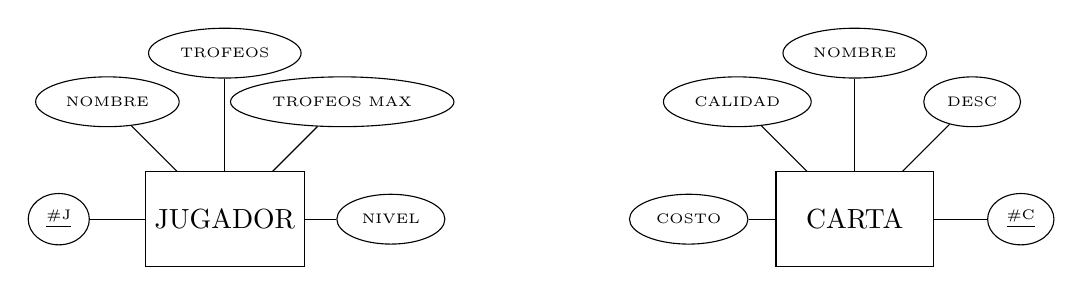
\begin{tikzpicture}[node distance=6em]
        \tikzstyle{every entity} = [minimum width=2cm, minimum height=1.2cm]
        \node[entity] (jugador) {JUGADOR}
            [sibling distance=3cm]
            child {node[attribute] [above right of=jugador] {\tiny TROFEOS MAX}}
            child {node[attribute] [above of=jugador] {\tiny TROFEOS}}
            child {node[attribute] [above left of=jugador] {\tiny NOMBRE}}
            child {node[attribute] [left of=jugador] {\underline{\tiny \#J}}}
            child {node[attribute] [right of=jugador] {\tiny NIVEL}}
            ;
       
        \node[entity] (carta) at (8,0) {CARTA}
        [sibling distance=3cm]
        child {node[attribute] [right of=carta] {\underline{\tiny \#C}}}
        child {node[attribute] [above of=carta] {\tiny NOMBRE}}
        child {node[attribute] [above left of=carta] {\tiny CALIDAD}}
        child {node[attribute] [above right of=carta] {\tiny DESC}}
        child {node[attribute] [left of=carta] {\tiny COSTO}};

    \end{tikzpicture}
    }\\[2mm]

    \begin{block}{}
        
        \hspace{20mm}Jugador(\underline{\#J}, Nombre, Nivel, Trofeos, TrofeosMax)\\
        \hspace{20mm}Carta(\underline{\#C}, Nombre, Calidad, Desc, Costo)\\
        
    \end{block}

    \note{@NOTE la llave primaria se subraya en la relaci\'on. Recuerden q puede ser compuesta}
\end{frame}


\begin{frame}{Relaciones para almacenar interrelaciones}
    \begin{block}{Llave for\'anea}
        Un conjunto de uno o m\'as atributos $F = \{A_1, A_2,...,A_n\}$ de una relaci\'on $R$, correspondientes
        a los dominios $D_1, D_2,...,D_n$ respectivamente, es una llave for\'anea referente a la relaci\'on $R'$ si:
        \begin{enumerate}
            \item La llave primaria de $R'$ es un conjunto de atributos $P = \{B_1,B_2,...,B_n\}$ correspondientes
            a los dominios $D_1,D_2,...,D_n$ respectivamente.
            \item Existe un acuerdo de correspondencia entre los atributos $A_i$ y $B_i$ para todo $i = 1,2,...,n$
           
        \end{enumerate}

        Una tupla $t \in R$ referencia a una tupla $t' \in R'$ si el valor de $A_i$ en la tupla $t$ es igual al valor
        de $B_i$ en la tupla $t'$ para todo $i=1,2,...,n$.
    \end{block}

\end{frame}

\begin{frame}{Interrelacionando registros: ejemplo}
    \begin{columns}[T]
        \begin{column}{0.48\linewidth}
            \begin{center}
                \vspace{10mm}
                \resizebox{\linewidth}{!}{
                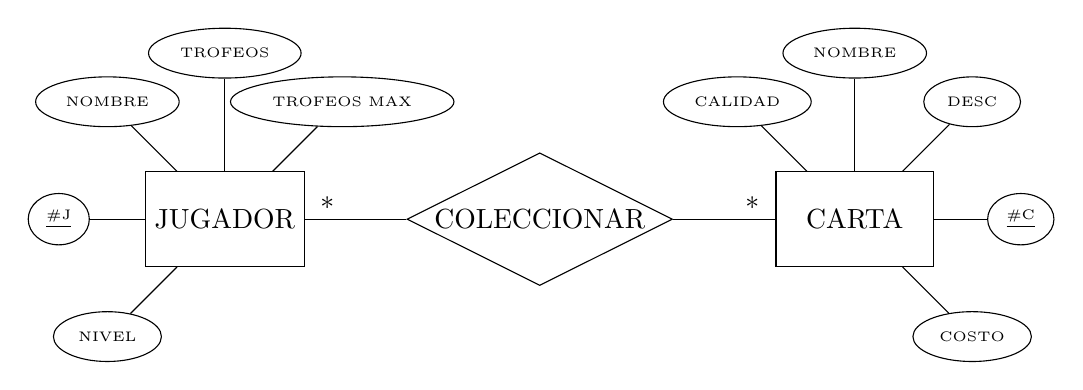
\begin{tikzpicture}[node distance=6em]
                    \tikzstyle{every entity} = [minimum width=2cm, minimum height=1.2cm]
                    \node[entity] (jugador) {JUGADOR}
                        [sibling distance=3cm]
                        child {node[attribute] [above right of=jugador] {\tiny TROFEOS MAX}}
                        child {node[attribute] [above of=jugador] {\tiny TROFEOS}}
                        child {node[attribute] [above left of=jugador] {\tiny NOMBRE}}
                        child {node[attribute] [left of=jugador] {\underline{\tiny \#J}}}
                        child {node[attribute] [below left of=jugador] {\tiny NIVEL}}
                        ;
                   
                    \node[entity] (carta) at (8,0) {CARTA}
                    [sibling distance=3cm]
                    child {node[attribute] [right of=carta] {\underline{\tiny \#C}}}
                    child {node[attribute] [above of=carta] {\tiny NOMBRE}}
                    child {node[attribute] [above left of=carta] {\tiny CALIDAD}}
                    child {node[attribute] [above right of=carta] {\tiny DESC}}
                    child {node[attribute] [below right of=carta] {\tiny COSTO}};

                    \node[relationship,aspect=2] (pertenecer) at (4,0) {COLECCIONAR}
                    edge(jugador) edge(carta);

                    \node at (1.3, 0.2) {$\ast$};
                    \node at (6.7, 0.2) {$\ast$};
                \end{tikzpicture}
                }
            \end{center}
        \end{column}

        \begin{column}{0.48\linewidth}
            \resizebox{\linewidth}{!}{
                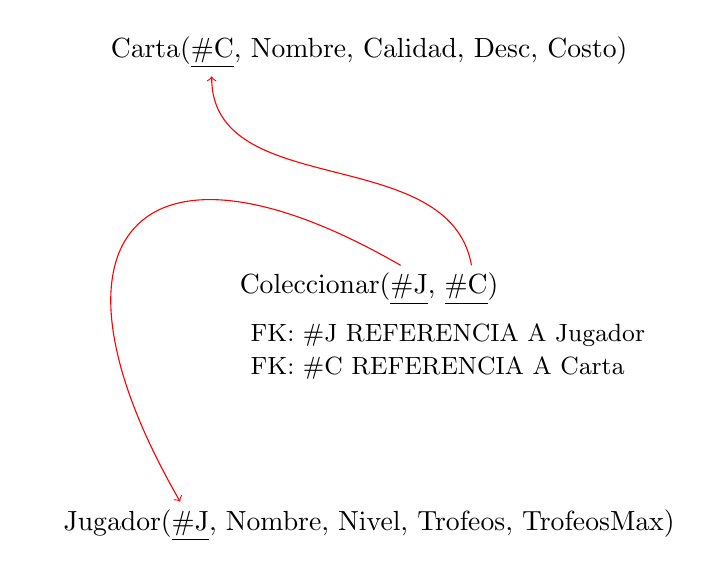
\begin{tikzpicture}
                    \node {Jugador(\underline{\#J}, Nombre, Nivel, Trofeos, TrofeosMax)};
                    \node at (0,6) {Carta(\underline{\#C}, Nombre, Calidad, Desc, Costo)};
                    \node at (0,3) { Coleccionar(\underline{\#J}, \underline{\#C})};
                    \node[align=left] at (1,2.2) {\small FK: \#J REFERENCIA A Jugador\\
                                                    \small FK: \#C REFERENCIA A Carta };

                    \path[->, color=red] (0.4,3.3) edge [out=150,in=120, looseness=2.4] (-2.4,0.3);
                    \path[->, color=red] (1.3,3.3) edge [out=100,in=270] (-2,5.7);
                    
                \end{tikzpicture}
            }
        \end{column}
        
    \end{columns}
    
    \note{@NOTE MUCHOS-MUCHOS}
\end{frame}


\begin{frame}{Interrelacionando registros: ejemplo}
    \begin{columns}[T]
        \begin{column}{0.48\linewidth}
            \centering
            \resizebox{\linewidth}{!}{
                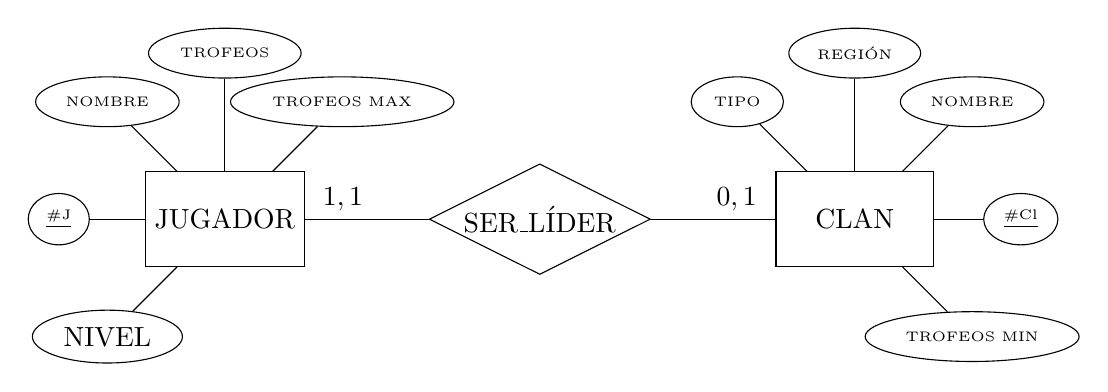
\begin{tikzpicture}[node distance=6em]
                    \tikzstyle{every entity} = [minimum width=2cm, minimum height=1.2cm]
                    \node[entity] (jugador) {JUGADOR}
                        [sibling distance=3cm]
                        child {node[attribute] [above right of=jugador] {\tiny TROFEOS MAX}}
                        child {node[attribute] [above of=jugador] {\tiny TROFEOS}}
                        child {node[attribute] [above left of=jugador] {\tiny NOMBRE}}
                        child {node[attribute] [left of=jugador] {\underline{\tiny \#J}}}
                        child {node[attribute] [below left of=jugador] {NIVEL}}
                        ;
                  
                    \node[entity] (clan) at (8,0) {CLAN}
                    [sibling distance=3cm]
                    child {node[attribute] [right of=clan] {\underline{\tiny \#Cl}}}
                    child {node[attribute] [above of=clan] {\tiny REGI\'ON}}
                    child {node[attribute] [above left of=clan] {\tiny TIPO}}
                    child {node[attribute] [above right of=clan] {\tiny NOMBRE}}
                    child {node[attribute] [below right of=clan] {\tiny TROFEOS MIN}};

                    \node[relationship,aspect=2] (pertenecer) at (4,0) {SER\_L\'IDER}
                    edge(jugador) edge(clan);

                    \node at (1.5, 0.25) {$1,1$};
                    \node at (6.5, 0.25) {$0,1$};
                \end{tikzpicture}
            }
        \end{column}

        \begin{column}{0.48\linewidth}
            \resizebox{\linewidth}{!}{
                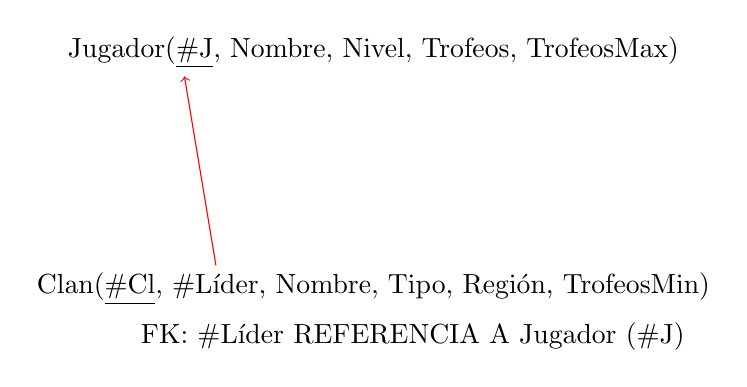
\begin{tikzpicture}
                    \node at (0,3){Jugador(\underline{\#J}, Nombre, Nivel, Trofeos, TrofeosMax)};
                    \node  {Clan(\underline{\#Cl}, \#L\'ider, Nombre, Tipo, Regi\'on, TrofeosMin)};
                    \node at (0.5,-0.6) {FK: \#L\'ider REFERENCIA A Jugador (\#J)};
                    \draw[->,color=red] (-2, 0.3) -- (-2.4,2.7);
                    
                \end{tikzpicture}
            }
        \end{column}
    \end{columns}
\end{frame}

\begin{frame}{Identificando relaciones}
    \begin{block}{Esquema de una relaci\'on}
        El esquema de una relaci\'on es una especificaci\'on de su estructura, la cual
        es independiente de las tuplas
        que contiene el cuerpo. El esquema se compone de: \begin{itemize}
            \item El nombre de la relaci\'on
            \item La cabecera
            \item La llave primaria
            \item Las llaves for\'aneas
        \end{itemize}
        En una misma base de datos una relaci\'on se identifica un\'ivocamente por su nombre.
    \end{block}

    \onslide<2>{
    \begin{block}{Instancia de una relaci\'on}
        Se refiere al conjunto de tuplas que constituye el cuerpo de la relaci\'on en un
        momento espec\'ifico del tiempo.
    \end{block}
    }
\end{frame}

\begin{frame}{Identificando relaciones: ejemplo}

    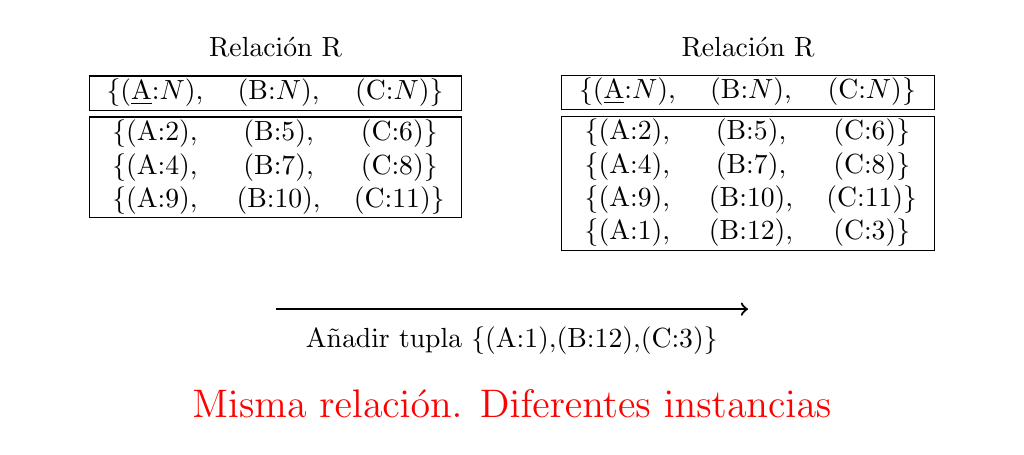
\begin{tikzpicture}
        \node at (0,0) {
            \begin{minipage}{0.50\textwidth}
                \centering
                Relaci\'on R\\[2mm]
                \begin{tabular}{|ccc|}
                    \hline
                    \{(\underline{A}:$\mathbb{N}$), & (B:$\mathbb{N}$), & (C:$\mathbb{N}$)\}\\
                    \hline
                    \hline
                    \{(A:2), & (B:5), & (C:6)\}\\
                    \{(A:4), & (B:7), & (C:8)\}\\
                    \{(A:9), & (B:10), & (C:11)\}\\
                    \hline
                \end{tabular}
            \end{minipage}    
        };
        \node at (6,-0.2) {
            \begin{minipage}{0.50\textwidth}
                \centering
                Relaci\'on R\\[2mm]
                \begin{tabular}{|ccc|}
                    \hline
                    \{(\underline{A}:$\mathbb{N}$), & (B:$\mathbb{N}$), & (C:$\mathbb{N}$)\}\\
                    \hline
                    \hline
                    \{(A:2), & (B:5), & (C:6)\}\\
                    \{(A:4), & (B:7), & (C:8)\}\\
                    \{(A:9), & (B:10), & (C:11)\}\\
                    \{(A:1), & (B:12), & (C:3)\}\\
                    \hline
                \end{tabular}
            \end{minipage}    
        };

        \draw[->,thick] (0,-2.3) -- (6,-2.3);

        \node at (3,-2.7) {A\~nadir tupla \{(A:1),(B:12),(C:3)\}};

        \node at (3,-3.5) {\Large \textcolor{red}{Misma relaci\'on. Diferentes instancias}};

    \end{tikzpicture}
\end{frame}


\begin{frame}{Modelo relacional}
    \vspace{5mm}
    \begin{overlayarea}{\linewidth}{\textheight}
        \begin{block}{Estructura de datos}
           Relaci\'on
        \end{block}
    \end{overlayarea}
\end{frame}


% \begin{frame}{Definiendo la abstracci\'on}

%     \hspace{8mm}\texttt{\kword{namespace} \tword{RelationalModel};}\\
%     \hspace{8mm}\texttt{\kword{using} \tword{RelationalTuple} = \tword{IDictionary}<\kword{string}, \kword{object}>;}\\[3mm]

%     \hspace{8mm}\texttt{\kword{public abstract class} \tword{Relation} \{ }\\[3mm]

%     \hspace{16mm}\texttt{\kword{public} \tword{IDictionary}<\kword{string}, \tword{Type}> Header \{\kword{get}; \kword{set};\}}\\
%     \hspace{16mm}\texttt{\kword{public} \tword{ISet}<\tword{RelationalTuple}> Body \{\kword{get}; \kword{set};\}}\\[3mm]

    
%     \hspace{16mm}\texttt{\kword{public} \tword{ISet}<\kword{string}> PrimaryKey \{\kword{get}; \kword{set};\}}\\
%     \hspace{16mm}\texttt{\kword{public} \tword{IDictionary}<\tword{Relation}, \tword{IDictionary}<\kword{string}, \kword{string}>> ForeignKeys \{\kword{get}; \kword{set};\}}\\
%     \hspace{8mm}\texttt{\}}
% \end{frame}







    \begin{frame}{Modelo relacional}
    \centering
    \Huge \textcolor{blue3}{Restricciones de integridad}
\end{frame}


\begin{frame}{¿Qu\'e es un estado consistente de la base de datos?}
    \begin{block}{Estado de una base de datos}
        \begin{itemize}
            \item  Conjunto de instancias $\{r_1,r_2,...,r_n\}$ de las relaciones $R_1,R_2,...,R_n$ respectivamente
            que conforman la base de datos en un instante de tiempo espec\'ifico.
            \item<2>  Un estado es consistente si satisface cada una de las restricciones de integridad
            definidas sobre la base de datos.
        \end{itemize}
       
    \end{block}
\end{frame}


% \begin{frame}{Metarreglas}
%     \begin{block}{Integridad de las entidades}
%         El valor de una llave primaria debe ser no nulo del todo 
%     \end{block}

%     \vspace{5mm}
%     \centering
%     \resizebox{!}{2.6cm}{
%         \begin{tikzpicture}[node distance=5em]
%             \tikzstyle{every entity} = [minimum width=2cm, minimum height=1.2cm]
%             \node[entity, double distance=1.5pt] (jugador) {TEMPORADA}
%                 [sibling distance=3cm]
%                 child {node[attribute] [above right of=jugador] {\tiny PREMIO}}
%                 child {node[attribute] [above of=jugador] {\tiny \underline{A\~NO}}}
%                 child {node[attribute] [above left of=jugador] {\tiny \underline{\#L}}}
%                 ;
          
%             \node[entity] (clan) at (8,0) {EQUIPO}
%             [sibling distance=3cm]
%             child {node[attribute] [above of=clan] {\tiny NOMBRE}}
%             child {node[attribute] [above left of=clan] {\tiny PA\'IS}}
%             child {node[attribute] [above right of=clan] {\tiny \underline{\#E}}};
%             \node[relationship,aspect=2] (pertenecer) at (4,0) {PARTICIPAR}
%             edge(jugador) edge(clan);
%         \end{tikzpicture}
%     }
% \end{frame}


\begin{frame}{\only<-3>{Metarreglas}\only<4>{La minimalidad}}
    \begin{block}{Integridad de las entidades}
        Todos los atributos de una llave primaria deben ser no nulos
    \end{block}
    \vspace{5mm}

    \begin{tikzpicture}
        \node at (0,0) {
            \begin{minipage}{0.50\textwidth}
                \centering
                Relaci\'on R\\[2mm]
                \begin{tabular}{|ccc|}
                    \hline
                    \{(\underline{A}:$\mathbb{N}$), & (\underline{B}:$\mathbb{N}$), & (C:$\mathbb{N}$)\}\\
                    \hline
                    \hline
                    \{({\color<3->{red}A:1}), & (B:2022), & (C:1000)\}\\
                    \{({\color<3->{red}A:1}), & (B:2021), & (C:1000)\}\\
                    \{(A:2), & (B:2022), & (C:1200)\}\\
                    \hline
                \end{tabular}
            \end{minipage}    
        };
        
        \onslide<2->{
            \node at (7.6, 0.2) {¿Se puede insertar esta tupla?};
            \node at (7.6,-0.3) {\{({\color<3->{red}A:1}),(B:NULL),(C:1000)\}};
        }
    \end{tikzpicture}
    \vspace{3mm}

    \centering
    \onslide<4>{
    \large \textcolor{red}{La llave es minimal. Si su valor est\'a incompleto entonces no es \'unico}
    }
\end{frame}

\begin{frame}{\only<-2>{Metarreglas}\only<3>{La minimalidad... otra vez}}
    \begin{block}{Integridad referencial}
        \begin{itemize}
            \item  Todos los atributos de una llave for\'anea deben ser no nulos o todos deben ser nulos.
            \item El valor de una llave for\'anea tiene que ser un valor existente de la llave primaria en la relaci\'on a la que hace referencia.
        \end{itemize}
    \end{block}

   \pause

    \begin{tikzpicture}
        \node at (0,0) {
            \begin{minipage}{0.50\textwidth}
                \centering
                Relaci\'on R\\[2mm]
                \begin{tabular}{|ccc|}
                    \hline
                    \{(\underline{A}:$\mathbb{N}$), & (\underline{B}:$\mathbb{N}$), & (C:$\mathbb{N}$)\}\\
                    \hline
                    \hline
                    \{(A:1), & ({\color<4>{red}B:2022}), & (C:1000)\}\\
                    \{(A:1), & (B:2021), & (C:1000)\}\\
                    \{(A:2), & ({\color<4>{red}B:2022}), & (C:1200)\}\\
                    \hline
                \end{tabular}
            \end{minipage}    
        };


        \node at (6.5,0) {
            \begin{minipage}{0.50\textwidth}
                \centering
                Relaci\'on S\\{\tiny FK: (A,B) REFERENCES R (A,B)}\\[2mm]
                \begin{tabular}{|ccc|}
                    \hline
                    \{(\underline{D}:$\mathbb{N}$), & (A:$\mathbb{N}$), & (B:$\mathbb{N}$)\}\\
                    \hline
                    \hline
                    \{(D:2), & (A:\only<2>{2}\only<3->{\textbf<3>{NULL}}), & ({\color<4>{red}B:2022})\}\\
                    \hline
                \end{tabular}
            \end{minipage}    
        };
        
    \end{tikzpicture}
    \vspace{3mm}

    \only<4>{
    \centering
    \large ¿A cu\'al tupla de la relaci\'on R referencia la tupla de la relaci\'on S?
    }

    \only<5>{
        \centering
        \large \textcolor{red}{El valor de una llave for\'anea es un valor de la llave primaria de otra tabla\\Tambi\'en le afecta la minimalidad.}}

\end{frame}


\begin{frame}{Metarreglas}
  

    \begin{block}{Integridad de los dominios}
        \begin{itemize}
            \item Todos los valores de un atributo de una
            relaci\'on tienen que provenir del dominio pertinente.
        \end{itemize}
        
    \end{block}
    \vspace{3mm}

    \centering
    \onslide<2>{
        \Large \textcolor{red}{Trivial}
    }

    \note<2>{@NOTE por qu\'e trivial? Poner contraejemplo.}

\end{frame}



\begin{frame}{Modelo relacional}
    \vspace{5mm}
    \begin{overlayarea}{\linewidth}{\textheight}
        \begin{block}{Estructura de datos}
           Relaci\'on
        \end{block}

        \begin{block}{Restricciones de integridad}
            \begin{itemize}
                \item Metarreglas
                \item Dependencias funcionales (\textit{spoiler})
                \item Restricciones del negocio (\textit{spoiler})
            \end{itemize}
            
        \end{block}
    \end{overlayarea}

    \note{@NOTE restricciones del negocio: todo no se puede representar hasta este punto (hay q programar)}
\end{frame}


    \begin{frame}{Modelo relacional}
    \centering
    \Huge \textcolor{blue3}{Operaciones}
\end{frame}

{
\setbeamertemplate{background} 
{
    
\includegraphics[width=\paperwidth,height=\paperheight]{img/events.jpg}
}
\begin{frame}
\end{frame}
}

\begin{frame}{Un modelo transaccional}
    \begin{block}{Transacciones}
        Una transacci\'on es un \textcolor{red}{conjunto de operaciones que
        modifican el estado de la base de datos} y:

        \begin{itemize}
            \item<2-> \textit{\textcolor{red}{\textbf{\it A}}tomicity}: Se considera como una sola operaci\'on, es decir, se
            realizan todos los cambios o no se realiza ninguno.
            \item<3-> \textit{\textcolor{red}{\textbf{\it C}}onsistency}: El estado de la base de datos es consistente antes y despu\'es de ejecutarse la transacci\'on, pudiendo no serlo durante la ejecuci\'on.
            \item<4-> \textit{\textcolor{red}{\textbf{\it I}}solation}: El estado intermedio de una transacci\'on no
            es visible por el resto de las transacciones: se aisla.
            \item<5-> \textit{\textcolor{red}{\textbf{\it D}}urability}: Luego de ejecutada la transacci\'on, los cambios
            de estado son persistentes y no pueden ser deshechos, incluso, en el caso
            de fallos del sistema.
        \end{itemize}
        
        \onslide<6>{
        \centering
        \Huge \textcolor{red}{Propiedades ACID}
        }
    \end{block}

    \note<3>{@NOTE no se puede acceder al estado durante la ejecuci\'on de una transacci\'on}
\end{frame}

\begin{frame}{Operaciones que modifican el estado}
    \begin{block}<2->{Insertar}
        \begin{enumerate}
            \item Debemos comprobar que todas las metarreglas se cumplan para la tupla que vamos a insertar.
        \end{enumerate}
    \end{block}

    \begin{block}<3->{Eliminar}
        \begin{enumerate}
            \item<4-> No tenemos que comprobar las metarreglas en la tupla que vamos a eliminar pues ya est\'a insertada
        \end{enumerate}
        
    \end{block}
    \vspace{3mm}

    \onslide<5>{
        \centering
         \textcolor{red}{¿Y si eliminamos un valor de llave primaria que es el valor de una llave for\'anea?}
    }
    
\end{frame}



\begin{frame}{Operaciones que modifican el estado}
    \begin{block}{Insertar}
        \begin{enumerate}
            \item Debemos comprobar que todas las metarreglas se cumplan para la tupla que vamos a insertar.
        \end{enumerate}
    \end{block}

    \begin{block}{Eliminar}
        \begin{enumerate}
            \item No tenemos que comprobar las metarreglas en la tupla que vamos a eliminar pues ya est\'a insertada
            \item La relaci\'on debe avisar al resto de las relaciones que un valor de la llave primaria se va a eliminar
            \item<2-> Las relaciones que referencian a la tupla eliminada tienen tres opciones: detener la eliminaci\'on, anular la llave for\'anea o eliminar las tuplas que utilicen dicho valor de llave for\'anea.
        \end{enumerate}
        
    \end{block}
    
\end{frame}


{
\setbeamertemplate{background} 
{
    
\includegraphics[width=\paperwidth,height=\paperheight]{img/delete.jpg}
}
\begin{frame}
\end{frame}
}

\begin{frame}{Operaciones que modifican el estado}
    \begin{block}{Actualizar}
      
    \end{block}

    \onslide<2>{
        \centering
        \textcolor{red}{
        Se puede ver como un proceso de insertar una tupla
        y eliminar una tupla.
        }
    }
\end{frame}

\begin{frame}{Operaciones que modifican el estado}
    \begin{block}{Actualizar}
        \begin{enumerate}
            \item Debemos hacer las comprobaciones pertinentes a la inserci\'on de la tupla modificada.
            \item<2-> Si el valor de la llave primaria se modifica debemos avisar al resto de las relaciones para que actualicen
            la llave for\'anea.
            \item<3-> Realizar una transacci\'on de dos operaciones: \begin{enumerate}
                \item Eliminar la tupla original
                \item Insertar la tupla modificada
            \end{enumerate}
        \end{enumerate}
        
    \end{block}
\end{frame}

\begin{frame}{Operaciones para responder preguntas}
    \begin{block}{\'Algebra relacional}  
    \end{block}

    % @NOTE q el a'lgebra relacional sirve para buscar
\end{frame}


{
\setbeamertemplate{background} 
{
    
\includegraphics[width=\paperwidth,height=\paperheight]{img/flashback.jpg}
}
\begin{frame}
\end{frame}
}


\begin{frame}{Operaciones para responder preguntas}
    \begin{block}{\'Algebra relacional}
        \begin{itemize}
            \item Lenguaje procedimental para el manejo y construcci\'on de relaciones.
            \item Compuesta por operandos (variables y relaciones) y operadores (extensi\'on
            de la Teor\'ia de conjuntos).
            \item Las operaciones del \'algebra relacional manipulan y producen
            relaciones (Propiedad relacional del cierre o clausura).
        \end{itemize}    
    \end{block}

\end{frame}


\begin{frame}{Asignaci\'on $(:=)$}

    La asignaci\'on se utiliza para destinar a una variable
    de relaci\'on el valor que se crea a partir de la aplicaci\'on
    de cualesquiera de las operaciones sobre las relaciones
    existentes.
\end{frame}


\begin{frame}{Renombrar}
    Operaci\'on que no afecta el conjunto de
    tuplas presentes en la relaci\'on sino que modifica
    el esquema de la relaci\'on. En espec\'ifico permite
    cambiar el nombre tanto de los atributos como el de la relaci\'on.
\end{frame}

\begin{frame}{Operaciones de Teor\'ia de conjuntos: Ejemplo}
    \centering
    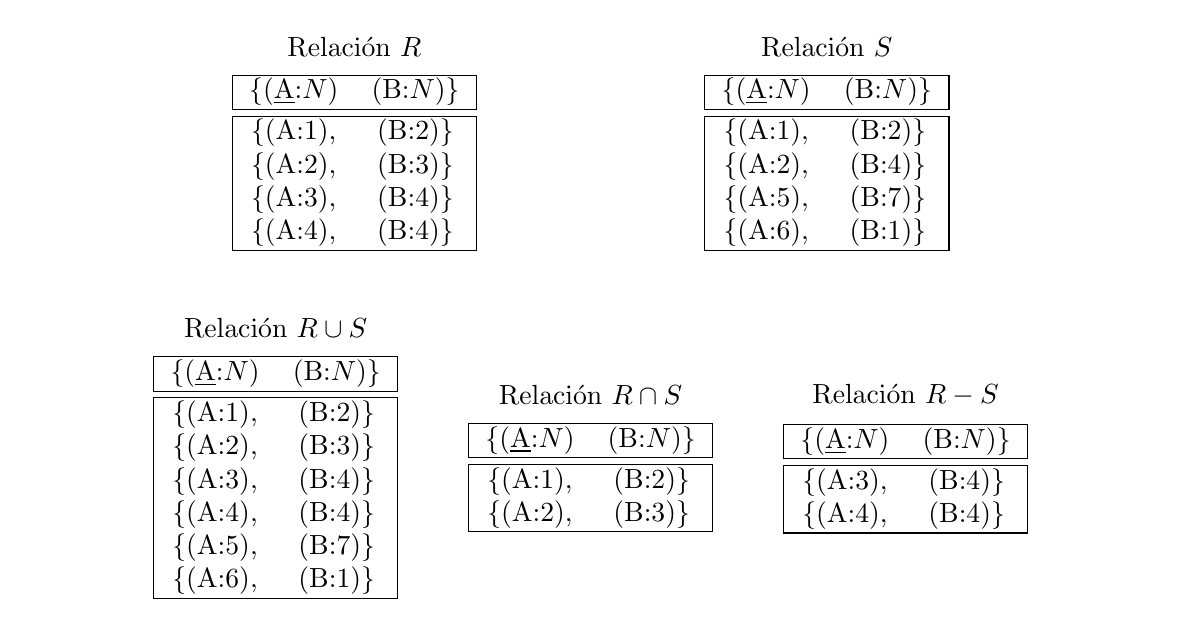
\begin{tikzpicture}
        \node at (0,0) {
            \begin{minipage}{0.50\textwidth}
                \centering
                Relaci\'on $R$\\[2mm]
                \begin{tabular}{|cc|}
                    \hline
                    \{(\underline{A}:$\mathbb{N}$) & (B:$\mathbb{N}$)\}\\
                    \hline
                    \hline
                    \{(A:1), &(B:2)\}\\
                    \{(A:2), &(B:3)\}\\
                    \{(A:3), &(B:4)\}\\
                    \{(A:4), &(B:4)\}\\
                    \hline
                \end{tabular}
            \end{minipage}    
        };

        \node at (6,0) {
            \begin{minipage}{0.50\textwidth}
                \centering
                Relaci\'on $S$\\[2mm]
                \begin{tabular}{|cc|}
                    \hline
                    \{(\underline{A}:$\mathbb{N}$) & (B:$\mathbb{N}$)\}\\
                    \hline
                    \hline
                    \{(A:1), &(B:2)\}\\
                    \{(A:2), &(B:4)\}\\
                    \{(A:5), &(B:7)\}\\
                    \{(A:6), &(B:1)\}\\
                    \hline
                \end{tabular}
            \end{minipage}    
        };

        \node at (-1,-4) {
            \begin{minipage}{0.50\textwidth}
                \centering
                Relaci\'on $R \cup S$\\[2mm]
                \begin{tabular}{|cc|}
                    \hline
                    \{(\underline{A}:$\mathbb{N}$) & (B:$\mathbb{N}$)\}\\
                    \hline
                    \hline
                    \{(A:1), &(B:2)\}\\
                    \{(A:2), &(B:3)\}\\
                    \{(A:3), &(B:4)\}\\
                    \{(A:4), &(B:4)\}\\
                    \{(A:5), &(B:7)\}\\
                    \{(A:6), &(B:1)\}\\
                    \hline
                \end{tabular}
            \end{minipage}    
        };

        \node at (3,-4) {
            \begin{minipage}{0.50\textwidth}
                \centering
                Relaci\'on $R \cap S$\\[2mm]
                \begin{tabular}{|cc|}
                    \hline
                    \{(\underline{A}:$\mathbb{N}$) & (B:$\mathbb{N}$)\}\\
                    \hline
                    \hline
                    \{(A:1), &(B:2)\}\\
                    \{(A:2), &(B:3)\}\\
                    \hline
                \end{tabular}
            \end{minipage}    
        };

        \node at (7,-4) {
            \begin{minipage}{0.50\textwidth}
                \centering
                Relaci\'on $R - S$\\[2mm]
                \begin{tabular}{|cc|}
                    \hline
                    \{(\underline{A}:$\mathbb{N}$) & (B:$\mathbb{N}$)\}\\
                    \hline
                    \hline
                    \{(A:3), &(B:4)\}\\
                    \{(A:4), &(B:4)\}\\
                    \hline
                \end{tabular}
            \end{minipage}    
        };

       

    \end{tikzpicture}

\end{frame}




% \begin{frame}{Intersecci\'on $(R \cap S)$}
%     Dadas dos relaciones $R$ y $S$ con la misma cabecera, la
%     intersecci\'on de dichas relaciones $(R \cap S)$ es una
%     relaci\'on del mismo tipo y con un cuerpo
%     que consiste en todas las tuplas que aparecen tanto en $R$ como en $S$.
% \end{frame}

% \begin{frame}{Diferencia $(R - S)$}
%     Dadas dos relaciones $R$ y $S$ con la misma cabecera, la
%     diferencia de dichas relaciones $(R - S)$ es una
%     relaci\'on del mismo tipo y con un cuerpo
%     que consiste en todas las tuplas que aparecen en $R$ y no en $S$. Esta
%     operaci\'on no es conmutativa.
% \end{frame}


\begin{frame}{Restricci\'on: Ejemplo }
    \centering
    \resizebox{15cm}{!}{
    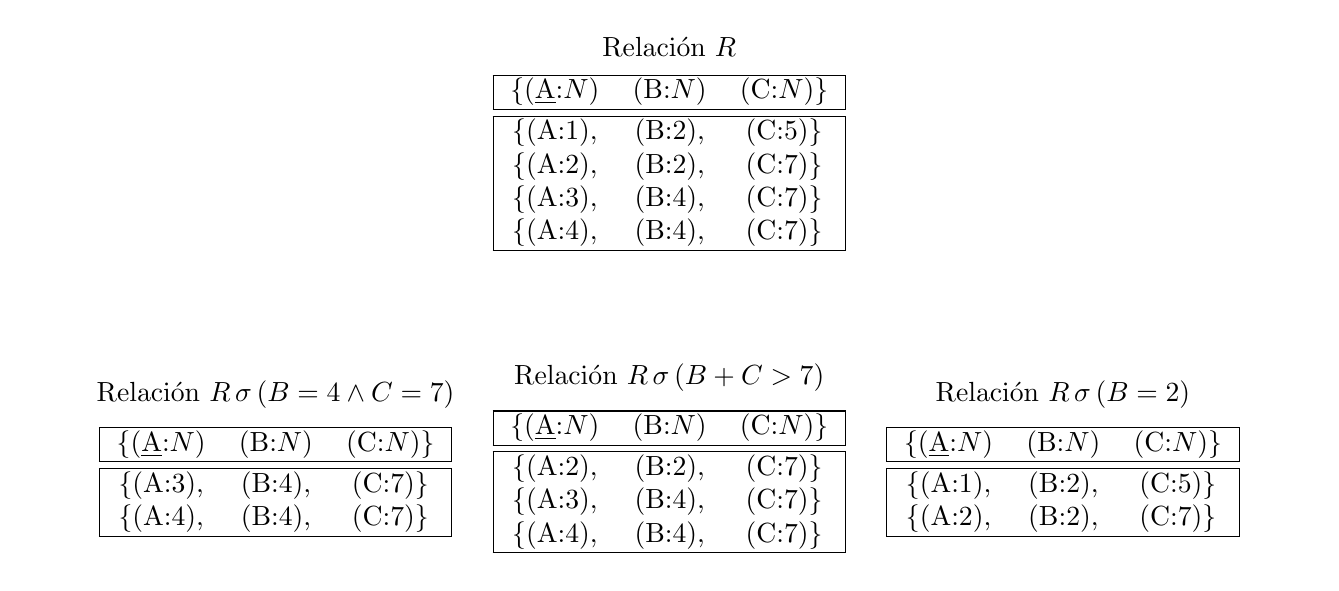
\begin{tikzpicture}
        \node at (0,0) {
            \begin{minipage}{0.50\textwidth}
                \centering
                Relaci\'on $R$\\[2mm]
                \begin{tabular}{|ccc|}
                    \hline
                    \{(\underline{A}:$\mathbb{N}$) & (B:$\mathbb{N}$)  & (C:$\mathbb{N}$)\}\\
                    \hline
                    \hline
                    \{(A:1), &(B:2),  & (C:5)\}\\
                    \{(A:2), &(B:2),  & (C:7)\}\\
                    \{(A:3), &(B:4),  & (C:7)\}\\
                    \{(A:4), &(B:4),  & (C:7)\}\\
                    \hline
                \end{tabular}
            \end{minipage}    
        };

        \node at (5,-4) {
            \begin{minipage}{0.50\textwidth}
                \centering
                Relaci\'on $R \,\sigma\, (B=2)$\\[2mm]
                \begin{tabular}{|ccc|}
                    \hline
                    \{(\underline{A}:$\mathbb{N}$) & (B:$\mathbb{N}$)  & (C:$\mathbb{N}$)\}\\
                    \hline
                    \hline
                    \{(A:1), &(B:2),  & (C:5)\}\\
                    \{(A:2), &(B:2),  & (C:7)\}\\
                    \hline
                \end{tabular}
            \end{minipage}    
        };


        \node at (0,-4) {
            \begin{minipage}{0.50\textwidth}
                \centering
                Relaci\'on $R \,\sigma\,(B + C > 7)$\\[2mm]
                \begin{tabular}{|ccc|}
                    \hline
                    \{(\underline{A}:$\mathbb{N}$) & (B:$\mathbb{N}$)  & (C:$\mathbb{N}$)\}\\
                    \hline
                    \hline
                    \{(A:2), &(B:2),  & (C:7)\}\\
                    \{(A:3), &(B:4),  & (C:7)\}\\
                    \{(A:4), &(B:4),  & (C:7)\}\\
                    \hline
                \end{tabular}
            \end{minipage}    
        };

        \node at (-5,-4) {
            \begin{minipage}{0.50\textwidth}
                \centering
                Relaci\'on $R \,\sigma\, (B =4 \land C=7)$\\[2mm]
                \begin{tabular}{|ccc|}
                    \hline
                    \{(\underline{A}:$\mathbb{N}$) & (B:$\mathbb{N}$)  & (C:$\mathbb{N}$)\}\\
                    \hline
                    \hline
                    \{(A:3), &(B:4),  & (C:7)\}\\
                    \{(A:4), &(B:4),  & (C:7)\}\\
                    \hline
                \end{tabular}
            \end{minipage}    
        };

      

        

       
    \end{tikzpicture}
    }

\end{frame}



\begin{frame}{Proyecci\'on: Ejemplo }
    \centering
    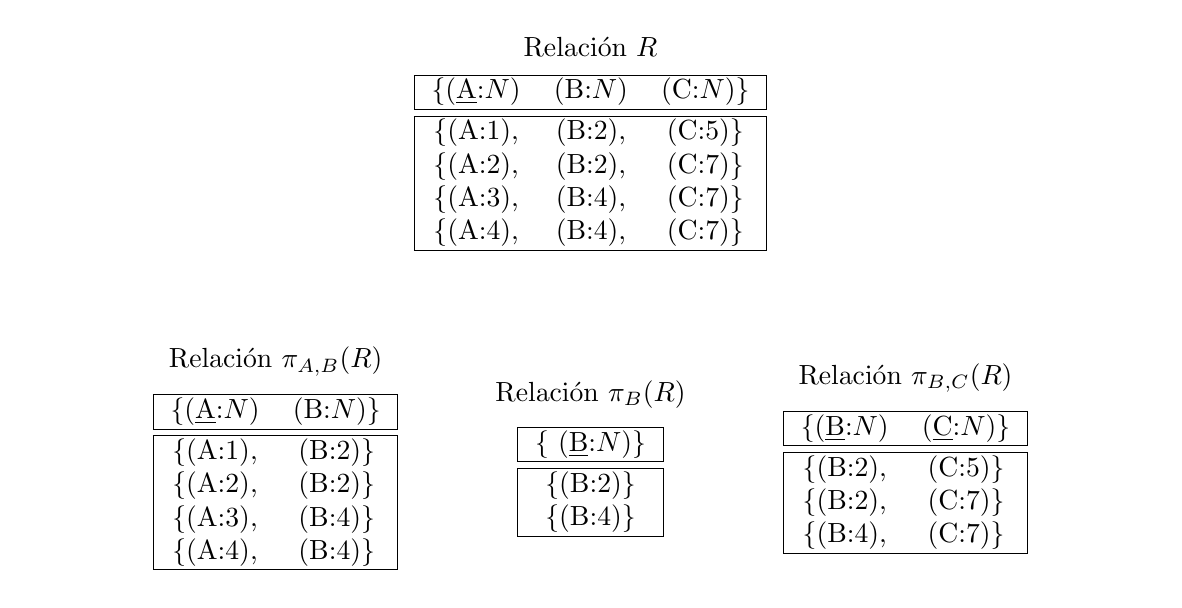
\begin{tikzpicture}
        \node at (0,0) {
            \begin{minipage}{0.50\textwidth}
                \centering
                Relaci\'on $R$\\[2mm]
                \begin{tabular}{|ccc|}
                    \hline
                    \{(\underline{A}:$\mathbb{N}$) & (B:$\mathbb{N}$)  & (C:$\mathbb{N}$)\}\\
                    \hline
                    \hline
                    \{(A:1), &(B:2),  & (C:5)\}\\
                    \{(A:2), &(B:2),  & (C:7)\}\\
                    \{(A:3), &(B:4),  & (C:7)\}\\
                    \{(A:4), &(B:4),  & (C:7)\}\\
                    \hline
                \end{tabular}
            \end{minipage}    
        };

        \node at (-4,-4) {
            \begin{minipage}{0.50\textwidth}
                \centering
                Relaci\'on $\pi_{A,B}(R)$\\[2mm]
                \begin{tabular}{|cc|}
                    \hline
                    \{(\underline{A}:$\mathbb{N}$) & (B:$\mathbb{N}$)\}\\
                    \hline
                    \hline
                    \{(A:1), &(B:2)\}\\
                    \{(A:2), &(B:2)\}\\
                    \{(A:3), &(B:4)\}\\
                    \{(A:4), &(B:4)\}\\
                    \hline
                \end{tabular}
            \end{minipage}    
        };

        \node at (0,-4) {
            \begin{minipage}{0.50\textwidth}
                \centering
                Relaci\'on $\pi_{B}(R)$\\[2mm]
                \begin{tabular}{|c|}
                    \hline
                    \{ (\underline{B}:$\mathbb{N}$)\}\\
                    \hline
                    \hline
                    \{(B:2)\}\\
                    \{(B:4)\}\\
                    \hline
                \end{tabular}
            \end{minipage}    
        };

        \node at (4,-4) {
            \begin{minipage}{0.50\textwidth}
                \centering
                Relaci\'on $\pi_{B,C}(R)$\\[2mm]
                \begin{tabular}{|cc|}
                    \hline
                    \{(\underline{B}:$\mathbb{N}$) & (\underline{C}:$\mathbb{N}$)\}\\
                    \hline
                    \hline
                    \{(B:2), &(C:5)\}\\
                    \{(B:2), &(C:7)\}\\
                    \{(B:4), &(C:7)\}\\
                    \hline
                \end{tabular}
            \end{minipage}    
        };

    \end{tikzpicture}

\end{frame}



\begin{frame}{Producto Cartesiano: Ejemplo}
    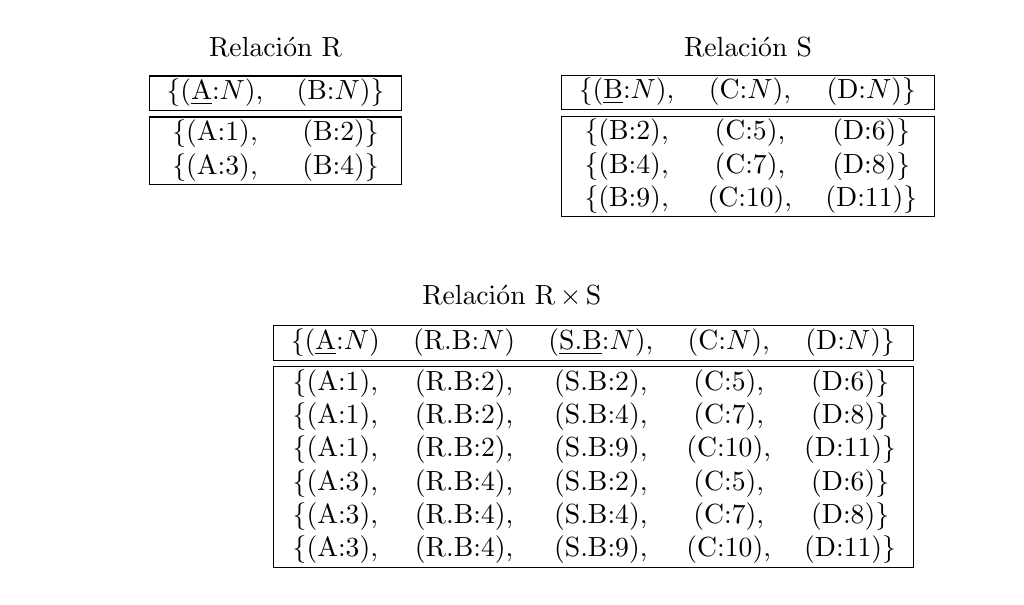
\begin{tikzpicture}
        \node {
            \begin{minipage}{0.50\textwidth}
                \centering
                Relaci\'on R\\[2mm]
                \begin{tabular}{|cc|}
                    \hline
                    \{(\underline{A}:$\mathbb{N}$), & (B:$\mathbb{N}$)\}\\
                    \hline
                    \hline
                    \{(A:1), & (B:2)\}\\
                    \{(A:3), & (B:4)\}\\
                    \hline
                \end{tabular}
            \end{minipage}    
        };


        \node at (6,-0.2) {
            \begin{minipage}{0.50\textwidth}
                \centering
                Relaci\'on S\\[2mm]
                \begin{tabular}{|ccc|}
                    \hline
                    \{(\underline{B}:$\mathbb{N}$), & (C:$\mathbb{N}$), & (D:$\mathbb{N}$)\}\\
                    \hline
                    \hline
                    \{(B:2), & (C:5), & (D:6)\}\\
                    \{(B:4), & (C:7), & (D:8)\}\\
                    \{(B:9), & (C:10), & (D:11)\}\\
                    \hline
                \end{tabular}
            \end{minipage}    
        };

        \onslide<2>{
        \node at (3,-4) {
            \begin{minipage}{0.50\textwidth}
                \centering
                Relaci\'on R$\,\times\,$S\\[2mm]
                \begin{tabular}{|ccccc|}
                    \hline
                    \{(\underline{A}:$\mathbb{N}$) & (R.B:$\mathbb{N}$) & (\underline{S.B}:$\mathbb{N}$), & (C:$\mathbb{N}$), & (D:$\mathbb{N}$)\}\\
                    \hline
                    \hline
                    \{(A:1), &(R.B:2), &(S.B:2), & (C:5), & (D:6)\}\\
                    \{(A:1), &(R.B:2), &(S.B:4), & (C:7), & (D:8)\}\\
                    \{(A:1), &(R.B:2), &(S.B:9), & (C:10), & (D:11)\}\\
                    \{(A:3), &(R.B:4), &(S.B:2), & (C:5), & (D:6)\}\\
                    \{(A:3), &(R.B:4), &(S.B:4), & (C:7), & (D:8)\}\\
                    \{(A:3), &(R.B:4), &(S.B:9), & (C:10), & (D:11)\}\\
                
                    \hline
                \end{tabular}
            \end{minipage}    
        };
        }
    \end{tikzpicture}
\end{frame}





\begin{frame}{Ya tenemos todas las operaciones que necesitamos...}
    \onslide<2>{
    \centering
    \Huge ...para poder definir el resto
    }

\end{frame}


\begin{frame}{Operaciones que combinan relaciones}
    \begin{block}{Natural Join $(R \Join S)$}
        Sean $R$ y $S$ dos relaciones, no necesariamente distintas, distinguimos
        los siguientes conjuntos de atributos:
        \begin{itemize}
            \item El conjunto $R_1,...,R_m$ son atributos de $R$ y no de $S$.
            \item El conjunto $S_1,...,S_n$ son atributos de $S$ y no de $R$.
            \item El conjunto $A_1,...,A_k$ son atributos comunes de $R$ y $S$, es decir, atributos
            con el mismo nombre y mismo dominio asociado en ambas relaciones. 
        \end{itemize}
        La operaci\'on $R \Join S$ \only<2>{\textcolor{red}{($R$ JOIN $S$)} }se define como:\\[2mm]
        \centering
        $
            \pi_{R_1,...,R_m,S_1,...,S_n,R.A_1,...,R.A_k}((R \times S)  \,\sigma\, (R.A_1 = S.A_1 \land ... \land R.A_k = S.A_k))
        $
    \end{block}

    \note<1>{@NOTE insistir en q 2 atributos no son =s si tienen dominios !=s, incluso cuan2 tengan nombres =s}
\end{frame}


\begin{frame}{Natural Join: Ejemplo}
    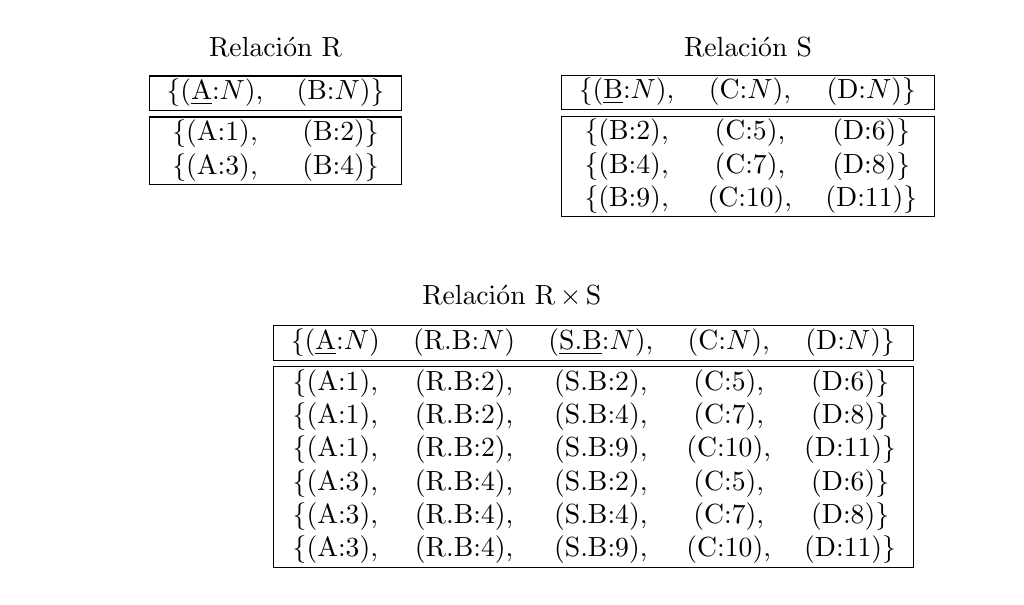
\begin{tikzpicture}
        \node {
            \begin{minipage}{0.50\textwidth}
                \centering
                Relaci\'on R\\[2mm]
                \begin{tabular}{|cc|}
                    \hline
                    \{(\underline{A}:$\mathbb{N}$), & (B:$\mathbb{N}$)\}\\
                    \hline
                    \hline
                    \{(A:1), & (B:2)\}\\
                    \{(A:3), & (B:4)\}\\
                    \hline
                \end{tabular}
            \end{minipage}    
        };


        \node at (6,-0.2) {
            \begin{minipage}{0.50\textwidth}
                \centering
                Relaci\'on S\\[2mm]
                \begin{tabular}{|ccc|}
                    \hline
                    \{(\underline{B}:$\mathbb{N}$), & (C:$\mathbb{N}$), & (D:$\mathbb{N}$)\}\\
                    \hline
                    \hline
                    \{(B:2), & (C:5), & (D:6)\}\\
                    \{(B:4), & (C:7), & (D:8)\}\\
                    \{(B:9), & (C:10), & (D:11)\}\\
                    \hline
                \end{tabular}
            \end{minipage}    
        };


        \node at (3,-4) {
            \begin{minipage}{0.50\textwidth}
                \centering
                Relaci\'on R$\,\times\,$S\\[2mm]
                \begin{tabular}{|ccccc|}
                    \hline
                    \{(\underline{A}:$\mathbb{N}$) & (R.B:$\mathbb{N}$) & (\underline{S.B}:$\mathbb{N}$), & (C:$\mathbb{N}$), & (D:$\mathbb{N}$)\}\\
                    \hline
                    \hline
                    \{(A:1), &(R.B:2), &(S.B:2), & (C:5), & (D:6)\}\\
                    \{(A:1), &(R.B:2), &(S.B:4), & (C:7), & (D:8)\}\\
                    \{(A:1), &(R.B:2), &(S.B:9), & (C:10), & (D:11)\}\\
                    \{(A:3), &(R.B:4), &(S.B:2), & (C:5), & (D:6)\}\\
                    \{(A:3), &(R.B:4), &(S.B:4), & (C:7), & (D:8)\}\\
                    \{(A:3), &(R.B:4), &(S.B:9), & (C:10), & (D:11)\}\\
                
                    \hline
                \end{tabular}
            \end{minipage}    
        };
    \end{tikzpicture}
\end{frame}

\begin{frame}{Natural Join: Ejemplo}
    \centering
    \begin{tikzpicture}
        \node at (0,0) {
            \begin{minipage}{0.50\textwidth}
                \centering
                \onslide<2->{{\color<3>{red}$F: R.B = S.B$}}\\[2mm]

                \centering
                Relaci\'on R$\,\times\,$S\\[2mm]
                \begin{tabular}{|ccccc|}
                    \hline
                    \{(\underline{A}:$\mathbb{N}$) & (R.B:$\mathbb{N}$) & (\underline{S.B}:$\mathbb{N}$), & (C:$\mathbb{N}$), & (D:$\mathbb{N}$)\}\\
                    \hline
                    \hline
                    \{(A:1), &{\color<3>{red}(R.B:2)}, &{\color<3>{red}(S.B:2)}, & (C:5), & (D:6)\}\\
                    \{(A:1), &(R.B:2), &(S.B:4), & (C:7), & (D:8)\}\\
                    \{(A:1), &(R.B:2), &(S.B:9), & (C:10), & (D:11)\}\\
                    \{(A:3), &(R.B:4), &(S.B:2), & (C:5), & (D:6)\}\\
                    \{(A:3), &{\color<3>{red}(R.B:4)}, &{\color<3>{red}(S.B:4)}, & (C:7), & (D:8)\}\\
                    \{(A:3), &(R.B:4), &(S.B:9), & (C:10), & (D:11)\}\\
                
                    \hline
                \end{tabular}
            \end{minipage}    
        };
    \end{tikzpicture}

\end{frame}


\begin{frame}{Natural Join: Ejemplo}
    \centering
    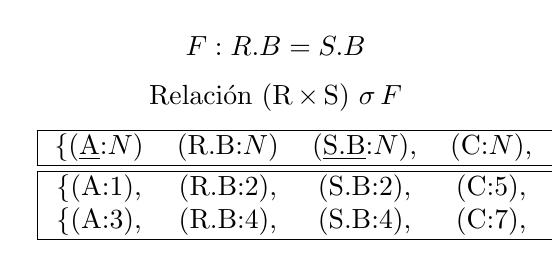
\begin{tikzpicture}
        \node at (0,0) {
            \begin{minipage}{0.50\textwidth}
                \centering
                $F: R.B = S.B$\\[2mm]

                \centering
                Relaci\'on (R$\,\times\,$S) $\sigma\, F$\\[2mm]
                \begin{tabular}{|ccccc|}
                    \hline
                    \{(\underline{A}:$\mathbb{N}$) & (R.B:$\mathbb{N}$) & (\underline{S.B}:$\mathbb{N}$), & (C:$\mathbb{N}$), & (D:$\mathbb{N}$)\}\\
                    \hline
                    \hline
                    \{(A:1), &(R.B:2), &(S.B:2), & (C:5), & (D:6)\}\\
                    \{(A:3), &(R.B:4), &(S.B:4), & (C:7), & (D:8)\}\\
                    \hline
                \end{tabular}
            \end{minipage}    
        };
    \end{tikzpicture}

\end{frame}



\begin{frame}{Natural Join: Ejemplo}
    \centering
    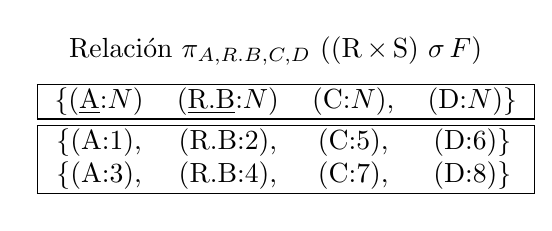
\begin{tikzpicture}
        \node at (0,0) {
            \begin{minipage}{0.50\textwidth}
                \centering
                Relaci\'on $\pi_{A,R.B,C,D}$ ((R$\,\times\,$S) $\sigma\, F$)\\[2mm]
                \begin{tabular}{|cccc|}
                    \hline
                    \{(\underline{A}:$\mathbb{N}$) & (\underline{R.B}:$\mathbb{N}$)  & (C:$\mathbb{N}$), & (D:$\mathbb{N}$)\}\\
                    \hline
                    \hline
                    \{(A:1), &(R.B:2),  & (C:5), & (D:6)\}\\
                    \{(A:3), &(R.B:4),  & (C:7), & (D:8)\}\\
                    \hline
                \end{tabular}
            \end{minipage}    
        };
    \end{tikzpicture}

\end{frame}


\begin{frame}{Natural Join: Ejemplo}
    \centering
    \begin{tikzpicture}
        \node at (0,0) {
            \begin{minipage}{0.50\textwidth}
                \centering
                Relaci\'on R $\Join$ S\\[2mm]
                \begin{tabular}{|cccc|}
                    \hline
                    \{(\underline{A}:$\mathbb{N}$) & (\underline{B}:$\mathbb{N}$)  & (C:$\mathbb{N}$), & (D:$\mathbb{N}$)\}\\
                    \hline
                    \hline
                    \{(A:1), &(B:2),  & (C:5), & (D:6)\}\\
                    \{(A:3), &(B:4),  & (C:7), & (D:8)\}\\
                    \hline
                \end{tabular}
            \end{minipage}    
        };
    \end{tikzpicture}

\end{frame}


\begin{frame}{Operaciones que combinan relaciones}
    \begin{block}{Theta Join ($\theta$-Join)}
        Sean $R$ y $S$ dos relaciones, no necesariamente distintas, definimos el
        $\theta$-Join de $R$ y $S$ como:

        $$
            (R \times S)\,\sigma\, F : F = \theta
        $$  

        donde $\theta$ es un condici\'on, expresada
        mediante una f\'ormula bien formada.
        
    \end{block}
\end{frame}

    \begin{frame}{Modelo relacional}
    \begin{overlayarea}{\linewidth}{\textheight}
        \begin{block}{Estructura de datos}
           Relaci\'on
        \end{block}

        \begin{block}{Restricciones de integridad}
            \begin{itemize}
                \item Metarreglas
                \item Dependencias funcionales (Spoiler)
                \item Restricciones del negocio (Spoiler)
            \end{itemize}
            
        \end{block}

        \begin{block}{Operaciones}
            \begin{itemize}
                \item Insertar
                \item Actualizar
                \item Eliminar
                \item \'Algebra relacional
            \end{itemize}
        \end{block}
    \end{overlayarea}

\end{frame}
    \begin{frame}{¿Qu\'e queremos?}
    \begin{columns}[T]
        \begin{column}{0.48\linewidth}
            \vspace{13mm}

            \resizebox{\linewidth}{!}{
                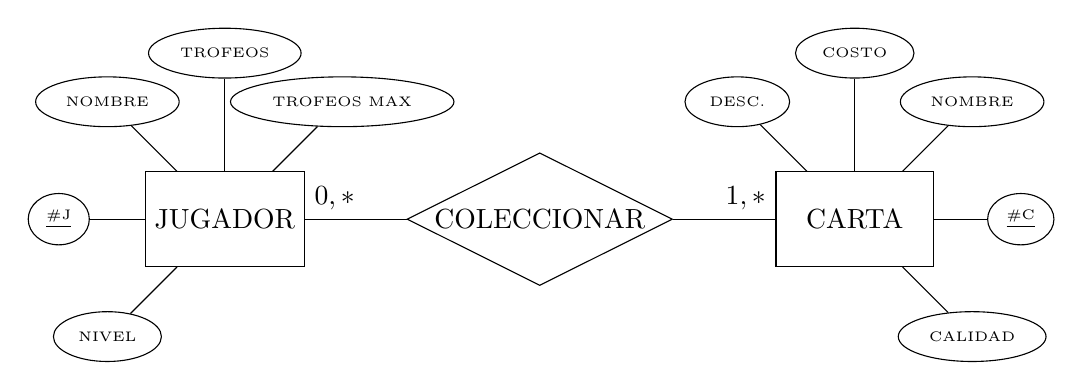
\begin{tikzpicture}[node distance=6em]
                    \tikzstyle{every entity} = [minimum width=2cm, minimum height=1.2cm]
                    \node[entity] (jugador) {JUGADOR}
                        [sibling distance=3cm]
                        child {node[attribute] [above right of=jugador] {\tiny TROFEOS MAX}}
                        child {node[attribute] [above of=jugador] {\tiny TROFEOS}}
                        child {node[attribute] [above left of=jugador] {\tiny NOMBRE}}
                        child {node[attribute] [left of=jugador] {\underline{\tiny \#J}}}
                        child {node[attribute] [below left of=jugador] {\tiny NIVEL}}
                        ;
                  
                    \node[entity] (clan) at (8,0) {CARTA}
                    [sibling distance=3cm]
                    child {node[attribute] [right of=clan] {\underline{\tiny \#C}}}
                    child {node[attribute] [above of=clan] {\tiny COSTO}}
                    child {node[attribute] [above left of=clan] {\tiny DESC.}}
                    child {node[attribute] [above right of=clan] {\tiny NOMBRE}}
                    child {node[attribute] [below right of=clan] {\tiny CALIDAD}};
                    
                  
                    \node[relationship,aspect=2] (pertenecer) at (4,0) {COLECCIONAR};
                    \draw (pertenecer.east) -- (clan.west) node[above left] {$1,\ast$};
                    \draw (pertenecer.west) -- (jugador.east) node[above right] {$0,\ast$};
                \end{tikzpicture}
            }
        \end{column}

        \begin{column}{0.48\linewidth}

           

                \vspace{14mm}

                \begin{scriptsize}
                    
                    \textbf{Jugador}(\underline{\#J}, Nombre, Nivel, Trofeos, TrofeosMax)\\[2mm]
                    \textbf{Carta}(\underline{\#C}, Nombre, Calidad, Desc., Costo)\\[2mm]
                    \textbf{Coleccionar}(\underline{\#J}, \underline{\#C})\\[1mm]
                    \hspace{4mm} FK: \#J REFERENCES Jugador\\
                    \hspace{4mm} FK: \#C REFERENCES Carta

                \end{scriptsize}

        \end{column}
        
    \end{columns}

\end{frame}

    \begin{frame}{Transformando el dise\~no}
    \centering
    \Huge \textcolor{blue3}{Dise\~no intuitivo}
\end{frame}

{
\setbeamertemplate{background} 
{
    
\includegraphics[width=\paperwidth,height=\paperheight]{img/algorithm.jpg}
}
\begin{frame}
\end{frame}
}


\begin{frame}{Ahora s\'i... transformando el dise\~no}
    \centering
    \Huge \textcolor{blue3}{Algoritmo del dise\~no intuitivo}
\end{frame}


\begin{frame}{Dise\~no intuitivo}
    \begin{block}<2->{La idea b\'asica}
        
        \begin{enumerate}
            \item<2-> Convertir cada conjunto de entidades en una relaci\'on con el mismo conjunto de atributos.
            
            \item<4-> Convertir cada interrelaci\'on en una relaci\'on cuyos atributos son las llaves primarias de las
            relaciones que representan los conjuntos de entidades conectados.
        \end{enumerate}
    \end{block}
    

    \begin{columns}[T]
        \begin{column}{0.48\linewidth}

            \resizebox{\linewidth}{!}{
                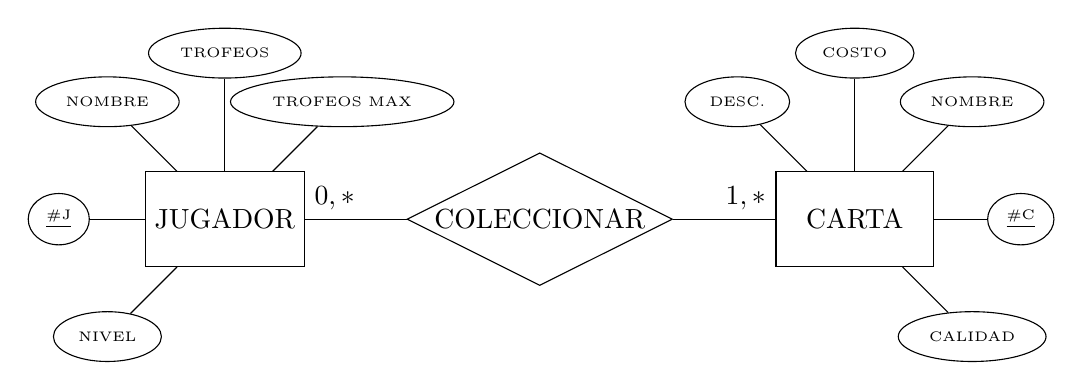
\begin{tikzpicture}[node distance=6em]
                    \tikzstyle{every entity} = [minimum width=2cm, minimum height=1.2cm]
                    \node[entity] (jugador) {JUGADOR}
                        [sibling distance=3cm]
                        child {node[attribute] [above right of=jugador] {\tiny TROFEOS MAX}}
                        child {node[attribute] [above of=jugador] {\tiny TROFEOS}}
                        child {node[attribute] [above left of=jugador] {\tiny NOMBRE}}
                        child {node[attribute] [left of=jugador] {\underline{\tiny \#J}}}
                        child {node[attribute] [below left of=jugador] {\tiny NIVEL}}
                        ;
                  
                    \node[entity] (clan) at (8,0) {CARTA}
                    [sibling distance=3cm]
                    child {node[attribute] [right of=clan] {\underline{\tiny \#C}}}
                    child {node[attribute] [above of=clan] {\tiny COSTO}}
                    child {node[attribute] [above left of=clan] {\tiny DESC.}}
                    child {node[attribute] [above right of=clan] {\tiny NOMBRE}}
                    child {node[attribute] [below right of=clan] {\tiny CALIDAD}};
                    
                  
                    \node[relationship,aspect=2] (pertenecer) at (4,0) {COLECCIONAR};
                    \draw (pertenecer.east) -- (clan.west) node[above left] {$1,\ast$};
                    \draw (pertenecer.west) -- (jugador.east) node[above right] {$0,\ast$};
                \end{tikzpicture}
            }
        \end{column}

        \begin{column}{0.48\linewidth}

        

                \begin{scriptsize}
                    \onslide<3->{
                        \textbf{Jugador}(\underline{\#J}, Nombre, Nivel, Trofeos, TrofeosMax)\\[2mm]
                        \textbf{Carta}(\underline{\#C}, Nombre, Calidad, Desc., Costo)\\[2mm]
                    }
                    \onslide<5->{
                        \textbf{Coleccionar}(\underline{\#J}, \underline{\#C})\\[1mm]
                        \hspace{4mm} FK: \#J REFERENCES Jugador\\
                        \hspace{4mm} FK: \#C REFERENCES Carta
                    }

                \end{scriptsize}

        \end{column}
        
    \end{columns}
\end{frame}



\begin{frame}{Aplicando el algoritmo}

    \begin{columns}[T]
        \begin{column}{0.48\linewidth}
            \centering
            \resizebox{\linewidth}{!}{
                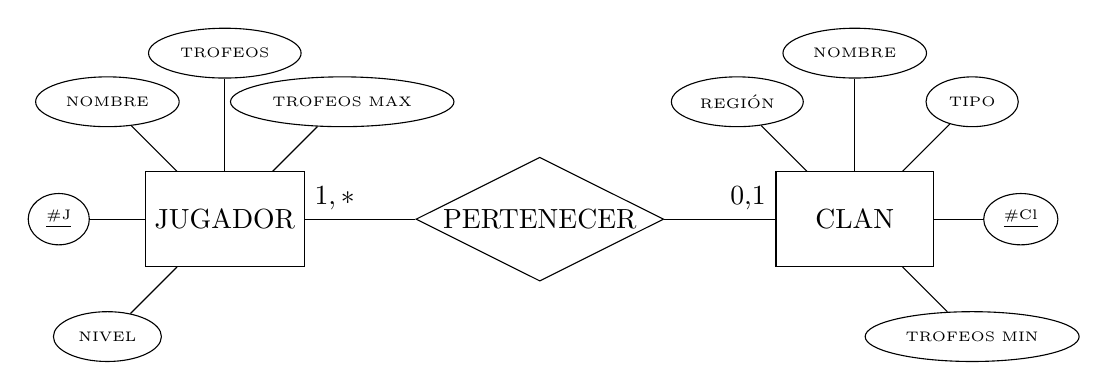
\begin{tikzpicture}[node distance=6em]
                    \tikzstyle{every entity} = [minimum width=2cm, minimum height=1.2cm]
                    \node[entity] (jugador) {JUGADOR}
                        [sibling distance=3cm]
                        child {node[attribute] [above right of=jugador] {\tiny TROFEOS MAX}}
                        child {node[attribute] [above of=jugador] {\tiny TROFEOS}}
                        child {node[attribute] [above left of=jugador] {\tiny NOMBRE}}
                        child {node[attribute] [left of=jugador] {\underline{\tiny \#J}}}
                        child {node[attribute] [below left of=jugador] {\tiny NIVEL}}
                        ;
                  
                    \node[entity] (clan) at (8,0) {CLAN}
                    [sibling distance=3cm]
                    child {node[attribute] [right of=clan] {\underline{\tiny \#Cl}}}
                    child {node[attribute] [above of=clan] {\tiny NOMBRE}}
                    child {node[attribute] [above left of=clan] {\tiny REGI\'ON}}
                    child {node[attribute] [above right of=clan] {\tiny TIPO}}
                    child {node[attribute] [below right of=clan] {\tiny TROFEOS MIN}};
                    
                  
                    \node[relationship,aspect=2] (pertenecer) at (4,0) {PERTENECER};
                    \draw (pertenecer.east) -- (clan.west) node[above left] {0,1};
                    \draw (pertenecer.west) -- (jugador.east)  node[above right] {$1, \ast$}; 
                \end{tikzpicture}
            }
        
        \end{column}

        \begin{column}{0.50\linewidth}
            \begin{scriptsize}
                \only<2-3>{
                    \textbf{Jugador}(\underline{\#J}, Nombre, Nivel, Trofeos, TrofeosMax)\\[2mm]
                    \textbf{Clan}(\underline{\#Cl}, Nombre, Regi\'on, Tipo, TrofeosMin)\\[2mm]
      
                    \textbf{Pertenecer}(\underline{\#J}, \underline{\#Cl})\\[1mm]
                    \hspace{4mm} FK: \#J REFERENCES Jugador\\[1mm]
                    \hspace{4mm} FK: \#Cl REFERENCES Clan
                }

        
            \end{scriptsize}
        \end{column}
        
    \end{columns}
   
    \vspace{10mm}
    \onslide<3>{
        \centering
        \textcolor{red}{\Large ¿Este dise\~no es eficiente?}


    }

    

\end{frame}


\begin{frame}{Un caso especial}

    \begin{columns}[T]
        \begin{column}{0.48\linewidth}
            \centering
            \resizebox{\linewidth}{!}{
                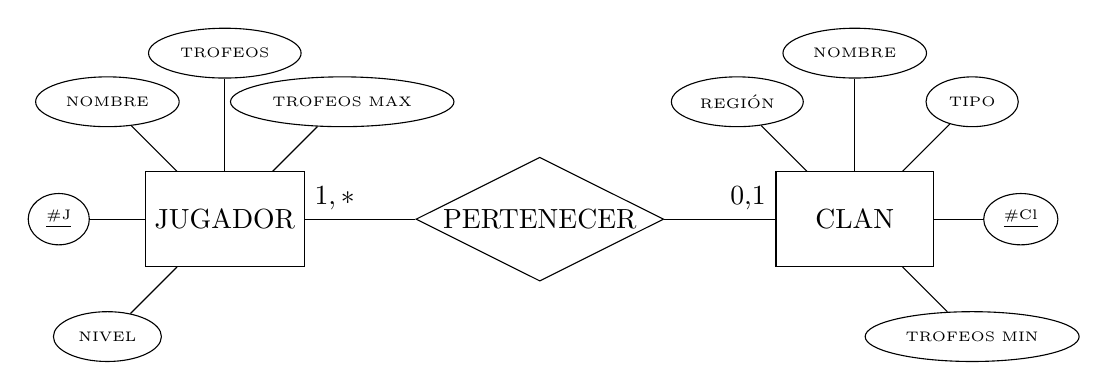
\begin{tikzpicture}[node distance=6em]
                    \tikzstyle{every entity} = [minimum width=2cm, minimum height=1.2cm]
                    \node[entity] (jugador) {JUGADOR}
                        [sibling distance=3cm]
                        child {node[attribute] [above right of=jugador] {\tiny TROFEOS MAX}}
                        child {node[attribute] [above of=jugador] {\tiny TROFEOS}}
                        child {node[attribute] [above left of=jugador] {\tiny NOMBRE}}
                        child {node[attribute] [left of=jugador] {\underline{\tiny \#J}}}
                        child {node[attribute] [below left of=jugador] {\tiny NIVEL}}
                        ;
                  
                    \node[entity] (clan) at (8,0) {CLAN}
                    [sibling distance=3cm]
                    child {node[attribute] [right of=clan] {\underline{\tiny \#Cl}}}
                    child {node[attribute] [above of=clan] {\tiny NOMBRE}}
                    child {node[attribute] [above left of=clan] {\tiny REGI\'ON}}
                    child {node[attribute] [above right of=clan] {\tiny TIPO}}
                    child {node[attribute] [below right of=clan] {\tiny TROFEOS MIN}};
                    
                  
                    \node[relationship,aspect=2] (pertenecer) at (4,0) {PERTENECER};
                    \draw (pertenecer.east) -- (clan.west) node[above left] {0,1};
                    \draw (pertenecer.west) -- (jugador.east)  node[above right] {$1, \ast$}; 
                \end{tikzpicture}
            }
        
        \end{column}

        \begin{column}{0.50\linewidth}
            \begin{scriptsize}


               
                    \vspace{5mm}
                    \textbf{Jugador}(\underline{\#J}, Nombre, Nivel, Trofeos, TrofeosMax, \#Cl)\\[1mm]
                    \hspace{4mm} FK: \#Cl REFERENCES Clan HAS NULL\\[2mm]
                    \textbf{Clan}(\underline{\#Cl}, Nombre, Regi\'on, Tipo, TrofeosMin)\\[2mm]
              
        
            \end{scriptsize}
        \end{column}
        
    \end{columns}
   
    \vspace{10mm}
    A\~nadir la llave primaria de la relaci\'on correspondiente al conjunto de entidades en el extremo con cardinalidad
            m\'axima \textcolor{red}{uno}
            a la relaci\'on correspondiente al conjunto de entidades en el otro extremo.
    

\end{frame}


\begin{frame}{Dise\~nos para interrelaciones de muchos a uno}
    \begin{columns}[T]
        \begin{column}{0.48\linewidth}
            \begin{scriptsize}
                \textbf{Jugador}(\underline{\#J}, Nombre, Nivel, Trofeos, TrofeosMax)\\[2mm]
                \textbf{Clan}(\underline{\#Cl}, Nombre, Regi\'on, Tipo, TrofeosMin)\\[2mm]
  
                \textbf{Pertenecer}(\underline{\#J}, \underline{\#Cl})\\[1mm]
                \hspace{4mm} FK: \#J REFERENCES Jugador\\
                \hspace{4mm} FK: \#Cl REFERENCES Clan
            \end{scriptsize}
        \end{column}

        \begin{column}{0.5\linewidth}
            \begin{scriptsize}
                \textbf{Jugador}(\underline{\#J}, Nombre, Nivel, Trofeos, TrofeosMax, \#Cl)\\[1mm]
                \hspace{4mm} FK: \#Cl REFERENCES Clan HAS NULL\\[2mm]
                \textbf{Clan}(\underline{\#Cl}, Nombre, Regi\'on, Tipo, TrofeosMin)\\[2mm]
            \end{scriptsize}
        \end{column}
        
    \end{columns}

    \vspace{5mm}

    \only<2>{
    \begin{center}
        \Large
        TAREA: ?`Cu\'ando uno es mejor que el otro?
    \end{center}
    }

    \note{@NOTE cu\'al es m\'as eficiente?}
\end{frame}

\begin{frame}{
    \only<1>{El caso especial del caso especial}
    \only<2>{Dise\~no para interrelaciones uno a uno: Opcionalidad}
    \only<3>{Dise\~no para interrelaciones uno a uno: Obligatoriedad}}

    \begin{columns}[T]
        \begin{column}{0.48\linewidth}
            \centering
            \resizebox{\linewidth}{!}{
                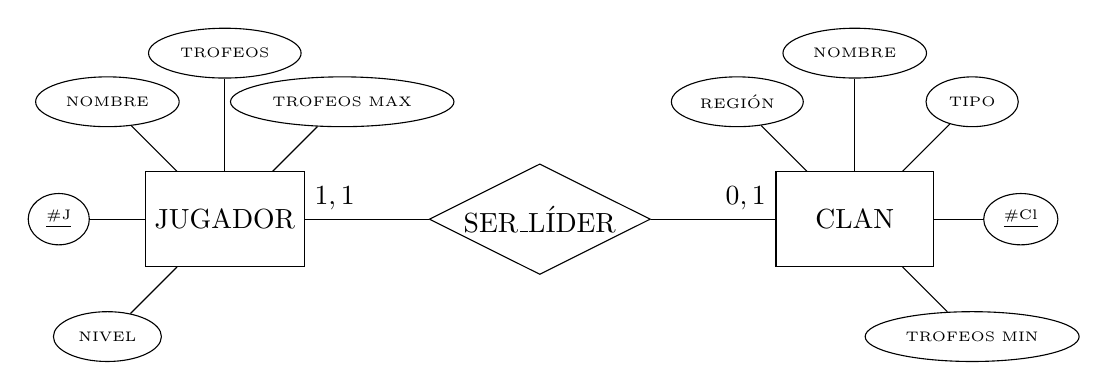
\begin{tikzpicture}[node distance=6em]
                    \tikzstyle{every entity} = [minimum width=2cm, minimum height=1.2cm]
                    \node[entity] (jugador) {JUGADOR}
                        [sibling distance=3cm]
                        child {node[attribute] [above right of=jugador] {\tiny TROFEOS MAX}}
                        child {node[attribute] [above of=jugador] {\tiny TROFEOS}}
                        child {node[attribute] [above left of=jugador] {\tiny NOMBRE}}
                        child {node[attribute] [left of=jugador] {\underline{\tiny \#J}}}
                        child {node[attribute] [below left of=jugador] {\tiny NIVEL}}
                        ;
                  
                    \node[entity] (clan) at (8,0) {CLAN}
                    [sibling distance=3cm]
                    child {node[attribute] [right of=clan] {\underline{\tiny \#Cl}}}
                    child {node[attribute] [above of=clan] {\tiny NOMBRE}}
                    child {node[attribute] [above left of=clan] {\tiny REGI\'ON}}
                    child {node[attribute] [above right of=clan] {\tiny TIPO}}
                    child {node[attribute] [below right of=clan] {\tiny TROFEOS MIN}};
                    
                  
                    \node[relationship,aspect=2] (pertenecer) at (4,0) {SER\_L\'IDER};
                    \draw (pertenecer.east) -- (clan.west) node[above left] {$0,1$};
                    \draw (pertenecer.west) -- (jugador.east)  node[above right] {$1, 1$}; 
                \end{tikzpicture}
            }
        
        \end{column}

        \begin{column}{0.50\linewidth}
            \begin{scriptsize}
                \only<2>{
                    \textbf{Jugador}(\underline{\#J}, Nombre, Nivel, Trofeos, TrofeosMax, \#Cl)\\[1mm]
                    \hspace{4mm} FK: \#Cl REFERENCES Clan HAS NULL\\[2mm]
                    \textbf{Clan}(\underline{\#Cl}, Nombre, Regi\'on, Tipo, TrofeosMin)\\[2mm]
                }

                \only<3>{
                    \vspace{5mm}
                    \textbf{Jugador}(\underline{\#J}, Nombre, Nivel, Trofeos, TrofeosMax)\\[1mm]
                    \textbf{Clan}(\underline{\#Cl}, Nombre, Regi\'on, Tipo, TrofeosMin, \#J)\\[1mm]
                    \hspace{4mm} FK: \#J REFERENCES Jugador\\[2mm]
                }
        
            \end{scriptsize}
        \end{column}

        
    \end{columns}
    
  
    

\end{frame}




\begin{frame}{Dise\~no para interrelaciones de uno a uno}

    \begin{columns}[T]
        \begin{column}{0.5\linewidth}
            \begin{scriptsize}
                
                \textbf{Jugador}(\underline{\#J}, Nombre, Nivel, Trofeos, TrofeosMax, \#Cl)\\[1mm]
                \hspace{4mm} FK: \#Cl REFERENCES Clan HAS NULL\\[2mm]
                \textbf{Clan}(\underline{\#Cl}, Nombre, Regi\'on, Tipo, TrofeosMin)\\[2mm]
            \end{scriptsize}
        \end{column}

        \begin{column}{0.48\linewidth}
            \begin{scriptsize}
                
                \textbf{Jugador}(\underline{\#J}, Nombre, Nivel, Trofeos, TrofeosMax)\\[1mm]
                \textbf{Clan}(\underline{\#Cl}, Nombre, Regi\'on, Tipo, TrofeosMin, \#J)\\[1mm]
                \hspace{4mm} FK: \#J REFERENCES Jugador\\[2mm]
            \end{scriptsize}
        \end{column}
        
    \end{columns}
    
    \vspace{5mm}

    \centering
    \large \textcolor{red}{Seleccionar el extremo con mayor cardinalidad m\'inima es m\'as eficiente}
    

\end{frame}


\begin{frame}{Dise\~no para interrelaciones con roles}
    \begin{columns}[T]

        \begin{column}{0.48\linewidth}
            \centering
            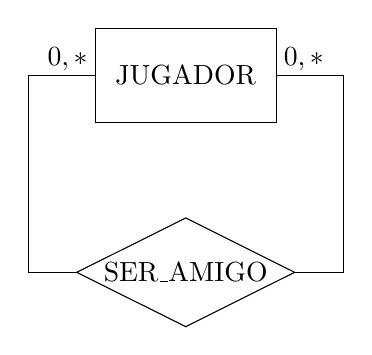
\begin{tikzpicture}
                \node[entity, minimum width=2.3cm, minimum height=1.2cm] (jugador) at (0,0) {JUGADOR};
                \node[relationship, aspect=2] (seramigo) at (0,-2.5) {SER\_AMIGO};
                \draw (seramigo.east) -- (2,-2.5) -- (2,0) -- (jugador.east);
                \draw (seramigo.west) -- (-2,-2.5) -- (-2,0) -- (jugador.west);
                \node at (-1.5,0.2) {$0 , \ast$};
                \node at (1.5,0.2) {$0,\ast$};
        
            \end{tikzpicture}
        \end{column}

        \begin{column}{0.48\linewidth}
            \vspace{15mm}
            \onslide<2->{

                \begin{scriptsize}
                    
                    \textbf{Ser\_Amigo}(\underline{\#Amigo1}, \underline{\#Amigo2})\\[1mm]
                    \hspace{4mm} FK: \#Amigo1 REFERENCES Jugador (\#J)\\[1mm]
                    \hspace{4mm} FK: \#Amigo2 REFERENCES Jugador (\#J)
                \end{scriptsize}
            }
        \end{column}
        
    \end{columns}
    \vspace{5mm}
    
    \onslide<3>{

        \centering
        \large \textcolor{red}{Se deben renombrar los atributos que tienen el mismo nombre}

    }

\end{frame}


\begin{frame}{Dise\~no para interrelaciones $n$-arias}
    \begin{columns}[T]
        \begin{column}{0.48\linewidth}
            \vspace{5mm}
            \centering
            \resizebox{\linewidth}{!}{
                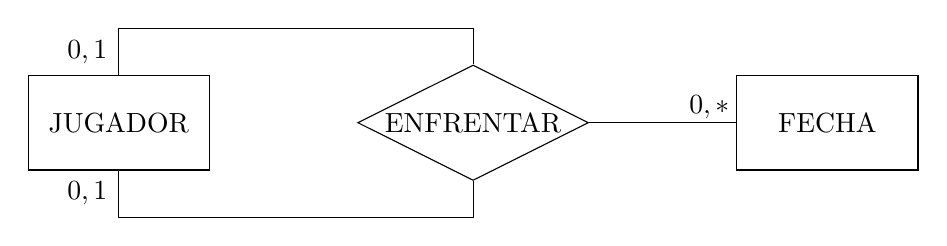
\begin{tikzpicture}
                    \tikzstyle{every entity} = [minimum width=2.3cm, minimum height=1.2cm]
                    \node[entity] (jugador) at (0,0) {JUGADOR};
                    \node[entity] (fecha) at (9,0) {FECHA};
                    \node[relationship, aspect=2] (enfrentar)at (4.5,0) {ENFRENTAR} edge(fecha);
                    \draw (jugador.south) -- (0,-1.2) -- (4.5,-1.2) -- (enfrentar.south); 
                    \draw (jugador.north) -- (0,1.2) -- (4.5,1.2) -- (enfrentar.north); 
            
                    \node at (-0.4,0.9) {$0,1$};
                    \node at (-0.4,-0.9) {$0,1$};
                    \node at (7.5,0.2) {$0,\ast$};
                \end{tikzpicture}
            }
        \end{column}

        \begin{column}{0.48\linewidth}
            \onslide<2->{

                \begin{scriptsize}
                    \textbf{Fecha}(\underline{Fecha})\\[2mm]
                    \textbf{Enfrentar}(\underline{\#J1}, \#J2, \underline{Fecha})\\[1mm]
                    \hspace{4mm}FK: \#J1 REFERENCES Jugador (\#J)\\[1mm]
                    \hspace{4mm}FK: \#J2 REFERENCES Jugador (\#J)\\[1mm]
                    \hspace{4mm}FK: Fecha REFERENCES Fecha\\[1mm]
                \end{scriptsize}
            }
        \end{column}
    \end{columns}
    
    \vspace{5mm}

    \onslide<3>{

        \begin{block}{}
            \begin{itemize}
                \item Convertir la interrelaci\'on en una relaci\'on cuyos atributos son las llaves primarias
                de las relaciones que representan los conjuntos de entidades conectados.
                \item   Si existen extremos
                de la interrelaci\'on con cardinalidad m\'axima uno, se escoge uno de ellos y su llave primaria
                se retira de la llave primaria de la relaci\'on resultante.
            \end{itemize}
        \end{block}
    }
        
     

   

   

\end{frame}

\begin{frame}{Dise\~no de agregaciones}
    \begin{columns}[T]
        \begin{column}{0.49\linewidth}
            \resizebox{\linewidth}{!}{
                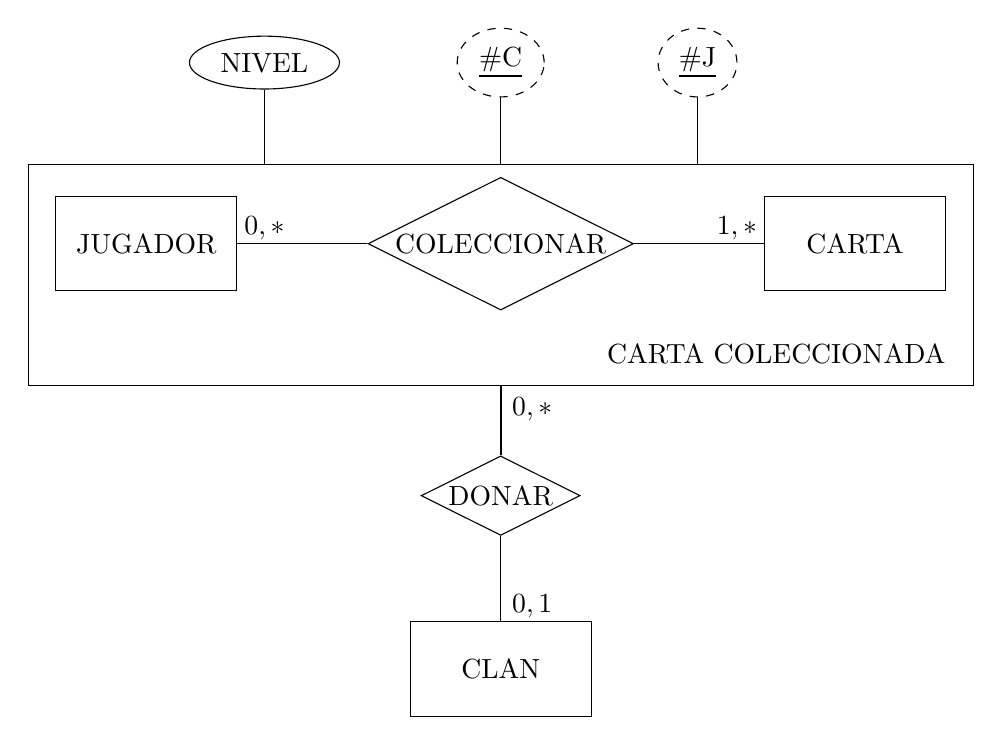
\begin{tikzpicture}
                    \tikzstyle{every entity} = [minimum width=2.3cm, minimum height=1.2cm]
                    \node[rectangle,draw,minimum width=12cm, minimum height=2.8cm] (coleccionada) at (4.5,-0.4) {};
                    \node[entity] (jugador) at (0,0) {JUGADOR};
                    \node[entity] (carta) at (9,0) {CARTA};
                    \node[relationship, aspect=2] (coleccionar) at (4.5,0) {COLECCIONAR} edge(jugador) edge(carta);
                    \node at (7.5,0.2) {$1,\ast$};
                    \node at (1.5,0.2) {$0,\ast$};
                    \node at (8,-1.4) {CARTA COLECCIONADA};
                    % \node[attribute] (nivel) at (4.5,2.3) { NIVEL};
                    % \draw[thick] (coleccionada.north) -- (nivel.south);

                    \node[entity] (clan) at (4.5,-5.4) {CLAN};
                    \node[relationship,aspect=2] (donar) at (4.5,-3.2) {DONAR} edge(clan);
                    \draw[thick] (coleccionada.south) -- (donar.north);
                    \node at (4.9, -2.1) {$0,\ast$};
                    \node at (4.9, -4.6) {$0,1$};

                    \node[attribute,dashed] (cartaid) at (4.5,2.3) { \underline{\#C}};
                    \node[attribute,dashed] (ci) at (7,2.3) {\underline{\#J}};
                    \node[attribute] (nivel) at (1.5,2.3) {NIVEL}; 
                    \draw (coleccionada.north) -- (cartaid.south);
                    \draw (7,1) -- (ci.south);
                    \draw (1.5,1) -- (nivel.south);
                \end{tikzpicture}
            }

        \end{column}

        \begin{column}{0.49\linewidth}
            \vspace{10mm}

            \onslide<2->{

                \begin{scriptsize}
                    
                    \textbf{Coleccionar}(\underline{\#J}, \underline{\#C}, \textcolor<3>{red}{Nivel})\\[2mm]
                    \textbf{Donar}(\underline{\#J}, \underline{\#C}, \underline{\#Cl})\\[1mm]
                    \hspace{2mm} FK: (\#J, \#C) REFERENCES Coleccionar (\#J, \#C)\\[1mm]
                    \hspace{2mm} FK: \#Cl REFERENCES Clan 
                    
                \end{scriptsize}
            }
        \end{column}
        
    \end{columns}
    \vspace{5mm}

    \onslide<3>{
        \centering
        \large \textcolor{red}{Agregar los atributos a la relaci\'on resultante de la interrelaci\'on}
        
    }
\end{frame}




\begin{frame}{Dise\~nos para la especializaci\'on}
    \begin{columns}[T]
        \begin{column}{0.40\linewidth}
            
            \centering
            \resizebox{\linewidth}{!}{
            \begin{tikzpicture}[node distance=5em]
                        \tikzset{link/.append style={
                    postaction={decorate},
                    decoration={
                        markings,
                        mark= at position 0.5 with {
                            \draw (0.5em,1ex) -- (-0.5em,1ex) to[bend right=90] (-0.5em,-1ex) -- (0.5em,-1ex);
                        }
                    }
                }}
                \tikzstyle{every entity} = [minimum width=2cm, minimum height=0.8cm]
        
                \node[entity] (jugador) {\small JUGADOR}
                    [sibling distance=3cm]
                    child {node[attribute] [above left of=jugador] {\tiny NIVEL}}
                    child {node[attribute] [above right of=jugador]{\tiny TROFEOS}}
                    child {node[attribute] [above of=jugador] {\tiny TROFEOS MAX}}
                    child {node[attribute] [right of=jugador]{\tiny NOMBRE}}
                    child {node[attribute] (ci) [left of=jugador] {\tiny \underline{\#J}}};
        
        
                \node[entity] (premium) at (-2,-3) {\small {\color<3->{blue}J. PREMIUM}}
                    [sibling distance=2.5cm]
                    child {node[attribute] [below left of=premium] {\tiny GASTO T.}}
                    child {node[attribute] [below right of=premium] {\tiny M. PAGO}}
                    child {node[attribute, dashed] [left of=premium] {\tiny \underline{\#J}}};
        
                \node[entity] (profesional) at (2,-3) {\small {\color<3->{orange}J. PROFESIONAL}}
                    [sibling distance=3.2cm]
                    child {node[attribute, dashed] [below left of=profesional] {\tiny \underline{\#J}}}
                    child {node[attribute] [below right of=profesional] {\tiny RANKING}};
        
                \draw[link] (premium.north) -- (-2,-1.3);
                \draw[link] (profesional.north) -- (2,-1.3);
                \draw (jugador.south) -- (0,-1.3);
                \draw (-2,-1.3) -- (0,-1.3);
                \draw (2,-1.3) -- (0,-1.3);
                % \draw[link] (premium.north) -- (jugador.south);
                % \draw[link] (profesional.north) -- (jugador.south);
        
                % \node[entity] (equipo) at (9,-3) {\small EQUIPO}
                % [sibling distance=3cm]
                % child {node[attribute] [above left of=equipo] {\tiny \underline{EQUIPO\_ID}}}
                % child {node[attribute] [above of=equipo] {\tiny NOMBRE}}
                % child {node[attribute] [above right of=equipo] {\tiny PA\'IS}};
                % \node[relationship, aspect=2] (miembro) at (5.8,-3) {\small MIEMBRO} edge(profesional) edge(equipo);
                % \node at (3.9,-2.8) {\small $1,\ast$};
                % \node at (7.6,-2.8) {\small $1,1$};
        
        
            \end{tikzpicture}
            }
        \end{column}

        \begin{column}{0.49\linewidth}
            \vspace{20mm}
            \onslide<2->{

                \begin{scriptsize}
                    
                    \textbf{Jugador}(\underline{\#J}, Nombre, Nivel, Trofeos, TrofeosMax, {\color<3->{blue}Gasto T.}, {\color<3->{blue}M. Pago}, {\color<3->{orange}Ranking})\\[2mm]
                \end{scriptsize}
            }
        \end{column}
        
    \end{columns}
    \vspace{5mm}

    \centering
    \onslide<4>{
        ¿Qu\'e ocurre si un jugador es profesional pero no premium?
    }
\end{frame}



\begin{frame}{Dise\~nos para la especializaci\'on}
    \begin{columns}[T]
        \begin{column}{0.40\linewidth}
            
            \centering
            \resizebox{\linewidth}{!}{
            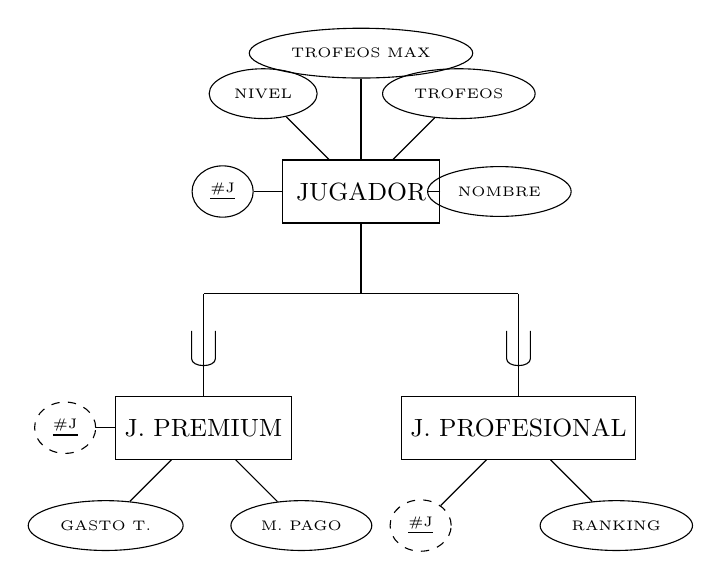
\begin{tikzpicture}[node distance=5em]
                        \tikzset{link/.append style={
                    postaction={decorate},
                    decoration={
                        markings,
                        mark= at position 0.5 with {
                            \draw (0.5em,1ex) -- (-0.5em,1ex) to[bend right=90] (-0.5em,-1ex) -- (0.5em,-1ex);
                        }
                    }
                }}
                \tikzstyle{every entity} = [minimum width=2cm, minimum height=0.8cm]
        
                \node[entity] (jugador) {\small JUGADOR}
                    [sibling distance=3cm]
                    child {node[attribute] [above left of=jugador] {\tiny NIVEL}}
                    child {node[attribute] [above right of=jugador]{\tiny TROFEOS}}
                    child {node[attribute] [above of=jugador] {\tiny TROFEOS MAX}}
                    child {node[attribute] [right of=jugador]{\tiny NOMBRE}}
                    child {node[attribute] (ci) [left of=jugador] {\tiny \underline{\#J}}};
        
        
                \node[entity] (premium) at (-2,-3) {\small J. PREMIUM}
                    [sibling distance=2.5cm]
                    child {node[attribute] [below left of=premium] {\tiny GASTO T.}}
                    child {node[attribute] [below right of=premium] {\tiny M. PAGO}}
                    child {node[attribute, dashed] [left of=premium] {\tiny \underline{\#J}}};
        
                \node[entity] (profesional) at (2,-3) {\small J. PROFESIONAL}
                    [sibling distance=3.2cm]
                    child {node[attribute, dashed] [below left of=profesional] {\tiny \underline{\#J}}}
                    child {node[attribute] [below right of=profesional] {\tiny RANKING}};
        
                \draw[link] (premium.north) -- (-2,-1.3);
                \draw[link] (profesional.north) -- (2,-1.3);
                \draw (jugador.south) -- (0,-1.3);
                \draw (-2,-1.3) -- (0,-1.3);
                \draw (2,-1.3) -- (0,-1.3);
                % \draw[link] (premium.north) -- (jugador.south);
                % \draw[link] (profesional.north) -- (jugador.south);
        
                % \node[entity] (equipo) at (9,-3) {\small EQUIPO}
                % [sibling distance=3cm]
                % child {node[attribute] [above left of=equipo] {\tiny \underline{EQUIPO\_ID}}}
                % child {node[attribute] [above of=equipo] {\tiny NOMBRE}}
                % child {node[attribute] [above right of=equipo] {\tiny PA\'IS}};
                % \node[relationship, aspect=2] (miembro) at (5.8,-3) {\small MIEMBRO} edge(profesional) edge(equipo);
                % \node at (3.9,-2.8) {\small $1,\ast$};
                % \node at (7.6,-2.8) {\small $1,1$};
        
        
            \end{tikzpicture}
            }
        \end{column}

        \begin{column}{0.49\linewidth}
            \vspace{15mm}
            \begin{scriptsize}
                
                \textbf{Jugador}(\underline{\#J}, Nombre, Nivel, Trofeos, TrofeosMax)\\[2mm]
                \textbf{J. Premium}(\underline{\#J}, Gasto T., M. Pago)\\[1mm]
                \hspace{4mm} FK: \#J REFERENCES Jugador\\[2mm]
                \textbf{J. Profesional}(\underline{\#J}, Ranking)\\[1mm]
                \hspace{4mm} FK: \#J REFERENCES Jugador
            \end{scriptsize}
        \end{column}
        
    \end{columns}
\end{frame}



\begin{frame}{Dise\~nos para la especializaci\'on}
    \begin{columns}[T]
        \begin{column}{0.48\linewidth}

            \begin{scriptsize}
                
                \textbf{Jugador}(\underline{\#J}, Nombre, Nivel, Trofeos, TrofeosMax, Gasto T., M. Pago, Ranking)\\[2mm]
            \end{scriptsize}
        \end{column}

        \begin{column}{0.48\linewidth}
            \begin{scriptsize}
                
                \textbf{Jugador}(\underline{\#J}, Nombre, Nivel, Trofeos, TrofeosMax)\\[2mm]
                \textbf{J. Premium}(\underline{\#J}, Gasto T., M. Pago)\\[1mm]
                \hspace{4mm} FK: \#J REFERENCES Jugador\\[2mm]
                \textbf{J. Profesional}(\underline{\#J}, Ranking)\\[1mm]
                \hspace{4mm} FK: \#J REFERENCES Jugador
            \end{scriptsize}
        \end{column}
        
    \end{columns}

    \note{@NOTE cu\'al es m\'as eficiente?}
\end{frame}



\begin{frame}{Dise\~nos para la especializaci\'on (partici\'on)}
    \begin{columns}[T]
        \begin{column}{0.48\linewidth}
            \resizebox{\linewidth}{!}{
    \begin{tikzpicture}[node distance=6em]
        \tikzset{link/.append style={
            postaction={decorate},
            decoration={
                markings,
                mark= at position 0.5 with {
                    \draw (0.5em,1ex) -- (-0.5em,1ex) to[bend right=90] (-0.5em,-1ex) -- (0.5em,-1ex);
                }
            }
        }}
        \tikzstyle{every entity} = [minimum width=2cm, minimum height=0.8cm]
        \node[entity] (carta) at (0,0) {CARTA}
        [sibling distance=3cm]
        child {node[attribute] [above left of=carta] {\tiny CALIDAD}}
        child {node[attribute] [above right of=carta]{\tiny DESC.}}
        child {node[attribute] [above of=carta] {\tiny NOMBRE}}
        child {node[attribute] [right of=carta]{\tiny COSTO}}
        child {node[attribute] [left of=carta] {\tiny \underline{CARTA\_ID}}};
        \node[regular polygon, draw, regular polygon sides=6, minimum width=7mm, xscale=3, label=center:TIPO] (tipo) at (0,-2) {};
        \draw (carta.south) -- (tipo.north);
        \node[entity] (tropa) at (0,-4.5) {{\color<2->{orange}TROPA}}
        [sibling distance=3cm]
        child {node[attribute, dashed] [above left of=tropa] {\tiny \underline{CARTA\_ID}}}
        child {node[attribute] [below of=tropa] {\tiny P. VIDA}}
        child {node[attribute] [below right of=tropa] {\tiny D. \'AREA}}
        child {node[attribute] [above right of=tropa] {\tiny UNIDADES}};
        \node[entity] (hechizo) at (-4,-4.5) {{\color<2->{blue}HECHIZO}}
        [sibling distance=3cm]
        child {node[attribute, dashed] [left of=hechizo] {\tiny \underline{CARTA\_ID}}}
        child {node[attribute] [below left of=hechizo] {\tiny RADIO}}
        child {node[attribute] [below of=hechizo] {\tiny DURACI\'ON}}
        child {node[attribute] [below right of=hechizo] {\tiny D. \'AREA}}
        child {node[attribute] [above left of=hechizo] {\tiny D. TORRES}};
        \node[entity] (estructura) at (3.4,-4.5) {{\color<2->{violet}ESTRUCTURA}}
        [sibling distance=3cm]
        child {node[attribute, dashed] [above right of=estructura] {\tiny \underline{CARTA\_ID}}}
        child {node[attribute] [right of=estructura] {\tiny D. DIST}}
        child {node[attribute] [below of=estructura] {\tiny V. ATAQUE}}
        child {node[attribute] [below right of=estructura] {\tiny P. VIDA}}
        ;
        \draw[link] (tropa.north) -- (tipo.south);
        \draw (-4,-2) -- (-1,-2);
        \draw[link] (hechizo.north) -- (-4,-2); 
        \draw (3.4,-2) -- (1,-2);
        \draw[link] (estructura.north) -- (3.4,-2);
    \end{tikzpicture}
    }
            
        \end{column}

        \begin{column}{0.48\linewidth}
            \vspace{20mm}

            \onslide<2->{

                \begin{scriptsize}
                    
                    \textbf{Carta}(\underline{\#C}, Nombre, Calidad, Desc., Costo, {\color<2->{blue}D.Torres}, {\color<2->{blue}Radio}, 
                    {\color<2->{blue}Duraci\'on}, {\color<2->{blue}H. D. \'Area}, {\color<2->{orange}Unidades}, {\color<2->{orange}T. P. Vida}, {\color<2->{orange}T. D. \'Area},
                    {\color<2->{violet}D. Dist}, {\color<2->{violet}E. P. Vida}, {\color<2->{violet}V. Ataque})
                \end{scriptsize}
            }
        \end{column}
        
    \end{columns}
    \vspace{5mm}

    \onslide<3>{

        \centering
        \large \textcolor{red}{Muy ineficiente espacialmente}
    }

    \note<3>{@NOTE por qu\'e?}
\end{frame}



\begin{frame}{Dise\~nos para la especializaci\'on (partici\'on)}
    \begin{columns}[T]
        \begin{column}{0.48\linewidth}
            \resizebox{\linewidth}{!}{
    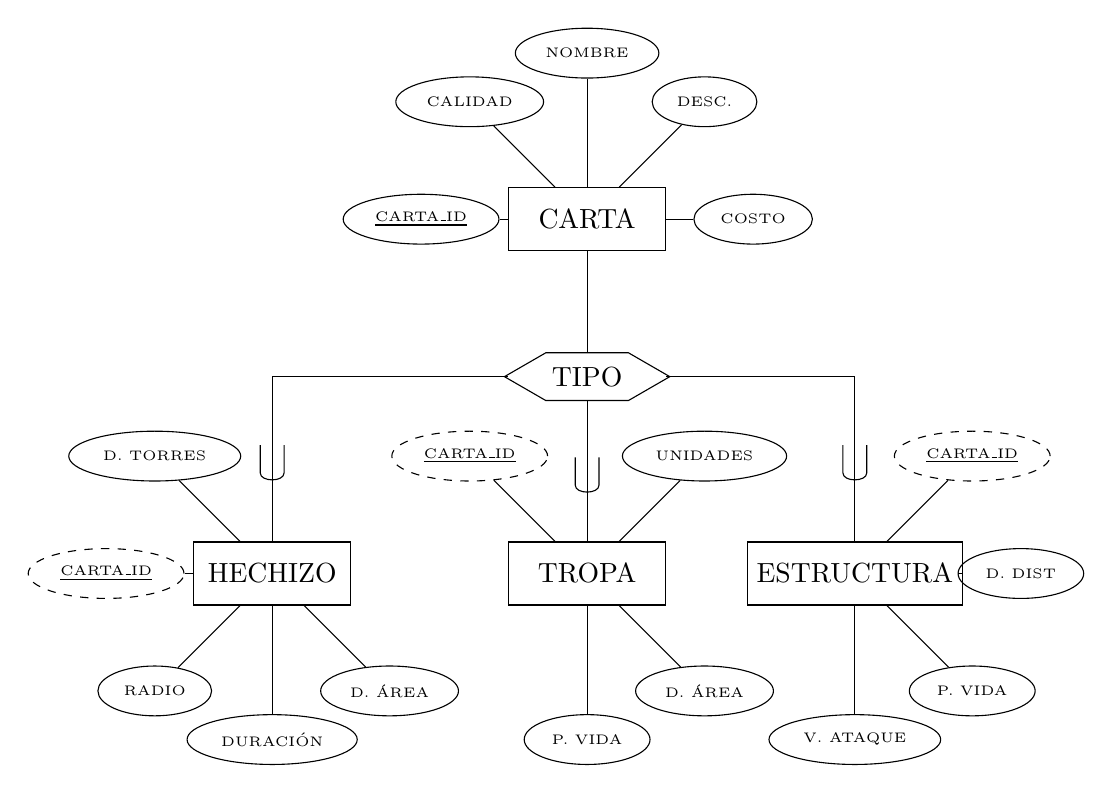
\begin{tikzpicture}[node distance=6em]
        \tikzset{link/.append style={
            postaction={decorate},
            decoration={
                markings,
                mark= at position 0.5 with {
                    \draw (0.5em,1ex) -- (-0.5em,1ex) to[bend right=90] (-0.5em,-1ex) -- (0.5em,-1ex);
                }
            }
        }}
        \tikzstyle{every entity} = [minimum width=2cm, minimum height=0.8cm]
        \node[entity] (carta) at (0,0) {CARTA}
        [sibling distance=3cm]
        child {node[attribute] [above left of=carta] {\tiny CALIDAD}}
        child {node[attribute] [above right of=carta]{\tiny DESC.}}
        child {node[attribute] [above of=carta] {\tiny NOMBRE}}
        child {node[attribute] [right of=carta]{\tiny COSTO}}
        child {node[attribute] [left of=carta] {\tiny \underline{CARTA\_ID}}};
        \node[regular polygon, draw, regular polygon sides=6, minimum width=7mm, xscale=3, label=center:TIPO] (tipo) at (0,-2) {};
        \draw (carta.south) -- (tipo.north);
        \node[entity] (tropa) at (0,-4.5) {TROPA}
        [sibling distance=3cm]
        child {node[attribute, dashed] [above left of=tropa] {\tiny \underline{CARTA\_ID}}}
        child {node[attribute] [below of=tropa] {\tiny P. VIDA}}
        child {node[attribute] [below right of=tropa] {\tiny D. \'AREA}}
        child {node[attribute] [above right of=tropa] {\tiny UNIDADES}};
        \node[entity] (hechizo) at (-4,-4.5) {HECHIZO}
        [sibling distance=3cm]
        child {node[attribute, dashed] [left of=hechizo] {\tiny \underline{CARTA\_ID}}}
        child {node[attribute] [below left of=hechizo] {\tiny RADIO}}
        child {node[attribute] [below of=hechizo] {\tiny DURACI\'ON}}
        child {node[attribute] [below right of=hechizo] {\tiny D. \'AREA}}
        child {node[attribute] [above left of=hechizo] {\tiny D. TORRES}};
        \node[entity] (estructura) at (3.4,-4.5) {ESTRUCTURA}
        [sibling distance=3cm]
        child {node[attribute, dashed] [above right of=estructura] {\tiny \underline{CARTA\_ID}}}
        child {node[attribute] [right of=estructura] {\tiny D. DIST}}
        child {node[attribute] [below of=estructura] {\tiny V. ATAQUE}}
        child {node[attribute] [below right of=estructura] {\tiny P. VIDA}}
        ;
        \draw[link] (tropa.north) -- (tipo.south);
        \draw (-4,-2) -- (-1,-2);
        \draw[link] (hechizo.north) -- (-4,-2); 
        \draw (3.4,-2) -- (1,-2);
        \draw[link] (estructura.north) -- (3.4,-2);
    \end{tikzpicture}
    }
            
        \end{column}

        \begin{column}{0.48\linewidth}
            \vspace{12mm}
            \begin{scriptsize}
                
                \textbf{Carta}(\underline{\#C}, Nombre, Calidad, Desc., Costo)\\[2mm]
                \textbf{Hechizo}(\underline{\#C}, D.Torres, Radio, Duraci\'on, D. \'Area)\\[1mm]
                \hspace{4mm} FK: \#C REFERENCES Carta \\[2mm]
                \textbf{Tropa}(\underline{\#C}, Unidades, P. Vida, D. \'Area)\\[1mm]
                \hspace{4mm} FK: \#C REFERENCES Carta \\[2mm]
                
                \textbf{Estructura}(\underline{\#C}, D. Dist, P. Vida, V. Ataque)\\[1mm]
                \hspace{4mm} FK: \#C REFERENCES Carta\\[2mm]
            \end{scriptsize}
        \end{column}
        
    \end{columns}


\end{frame}


\begin{frame}{Dise\~nos para la especializaci\'on (partici\'on)}
    \begin{columns}[T]
        \begin{column}{0.48\linewidth}
            \resizebox{\linewidth}{!}{
    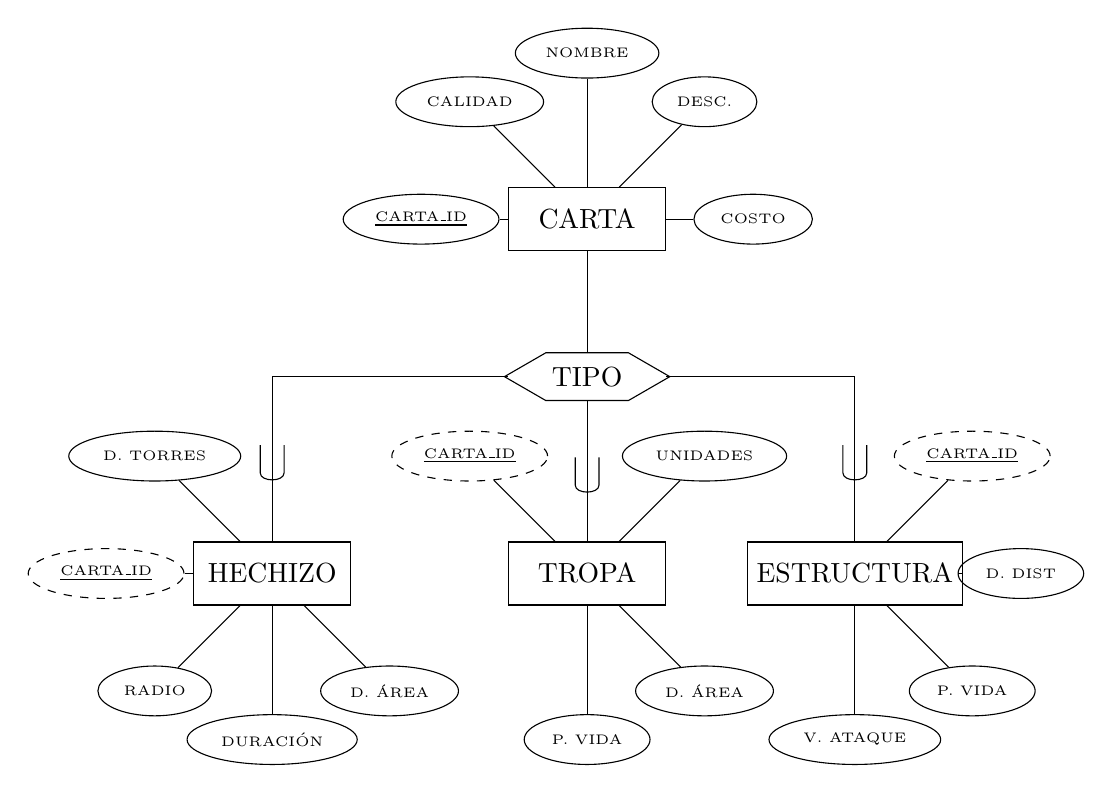
\begin{tikzpicture}[node distance=6em]
        \tikzset{link/.append style={
            postaction={decorate},
            decoration={
                markings,
                mark= at position 0.5 with {
                    \draw (0.5em,1ex) -- (-0.5em,1ex) to[bend right=90] (-0.5em,-1ex) -- (0.5em,-1ex);
                }
            }
        }}
        \tikzstyle{every entity} = [minimum width=2cm, minimum height=0.8cm]
        \node[entity] (carta) at (0,0) {CARTA}
        [sibling distance=3cm]
        child {node[attribute] [above left of=carta] {\tiny CALIDAD}}
        child {node[attribute] [above right of=carta]{\tiny DESC.}}
        child {node[attribute] [above of=carta] {\tiny NOMBRE}}
        child {node[attribute] [right of=carta]{\tiny COSTO}}
        child {node[attribute] [left of=carta] {\tiny \underline{CARTA\_ID}}};
        \node[regular polygon, draw, regular polygon sides=6, minimum width=7mm, xscale=3, label=center:TIPO] (tipo) at (0,-2) {};
        \draw (carta.south) -- (tipo.north);
        \node[entity] (tropa) at (0,-4.5) {TROPA}
        [sibling distance=3cm]
        child {node[attribute, dashed] [above left of=tropa] {\tiny \underline{CARTA\_ID}}}
        child {node[attribute] [below of=tropa] {\tiny P. VIDA}}
        child {node[attribute] [below right of=tropa] {\tiny D. \'AREA}}
        child {node[attribute] [above right of=tropa] {\tiny UNIDADES}};
        \node[entity] (hechizo) at (-4,-4.5) {HECHIZO}
        [sibling distance=3cm]
        child {node[attribute, dashed] [left of=hechizo] {\tiny \underline{CARTA\_ID}}}
        child {node[attribute] [below left of=hechizo] {\tiny RADIO}}
        child {node[attribute] [below of=hechizo] {\tiny DURACI\'ON}}
        child {node[attribute] [below right of=hechizo] {\tiny D. \'AREA}}
        child {node[attribute] [above left of=hechizo] {\tiny D. TORRES}};
        \node[entity] (estructura) at (3.4,-4.5) {ESTRUCTURA}
        [sibling distance=3cm]
        child {node[attribute, dashed] [above right of=estructura] {\tiny \underline{CARTA\_ID}}}
        child {node[attribute] [right of=estructura] {\tiny D. DIST}}
        child {node[attribute] [below of=estructura] {\tiny V. ATAQUE}}
        child {node[attribute] [below right of=estructura] {\tiny P. VIDA}}
        ;
        \draw[link] (tropa.north) -- (tipo.south);
        \draw (-4,-2) -- (-1,-2);
        \draw[link] (hechizo.north) -- (-4,-2); 
        \draw (3.4,-2) -- (1,-2);
        \draw[link] (estructura.north) -- (3.4,-2);
    \end{tikzpicture}
    }
            
        \end{column}

        \begin{column}{0.48\linewidth}
            \vspace{12mm}
            \begin{scriptsize}
                \textbf{Hechizo}(\underline{\#C}, Nombre, Calidad, Desc., Costo, D.Torres, Radio, Duraci\'on, D. \'Area)\\[1mm]
               
                \textbf{Tropa}(\underline{\#C}, Nombre, Calidad, Desc., Costo, Unidades, P. Vida, D. \'Area)\\[1mm]
                \textbf{Estructura}(\underline{\#C}, Nombre, Calidad, Desc., Costo, D. Dist, P. Vida, V. Ataque)\\[1mm]
            \end{scriptsize}
        \end{column}
        
    \end{columns}


\end{frame}


\begin{frame}{Dise\~nos para la especializaci\'on (partici\'on)}

    \begin{columns}[T]

        \begin{column}{0.48\linewidth}
            \begin{scriptsize}
                
                \textbf{Carta}(\underline{\#C}, Nombre, Calidad, Desc., Costo)\\[2mm]
                \textbf{Hechizo}(\underline{\#C}, D.Torres, Radio, Duraci\'on, D. \'Area)\\[1mm]
                \hspace{4mm} FK: \#C REFERENCES Carta \\[2mm]
                \textbf{Tropa}(\underline{\#C}, Unidades, P. Vida, D. \'Area)\\[1mm]
                \hspace{4mm} FK: \#C REFERENCES Carta \\[2mm]
                
                \textbf{Estructura}(\underline{\#C}, D. Dist, P. Vida, V. Ataque)\\[1mm]
                \hspace{4mm} FK: \#C REFERENCES Carta\\[2mm]
            \end{scriptsize}
        \end{column}

        \begin{column}{0.48\linewidth}

            \begin{scriptsize}
                \textbf{Hechizo}(\underline{\#C}, Nombre, Calidad, Desc., Costo, D.Torres, Radio, Duraci\'on, D. \'Area)\\[1mm]
               
                \textbf{Tropa}(\underline{\#C}, Nombre, Calidad, Desc., Costo, Unidades, P. Vida, D. \'Area)\\[1mm]
               
                \textbf{Estructura}(\underline{\#C}, Nombre, Calidad, Desc., Costo, D. Dist, P. Vida, V. Ataque)\\[1mm]
             
            \end{scriptsize}
        \end{column}
        
    \end{columns}

    \vspace{5mm}

    \only<2>{
    \begin{center}
        \Large
        TAREA: ?`Cu\'ando uno es mejor que el otro?
    \end{center}
    }

    \note{@NOTE cu\'al es m\'as eficiente?}
\end{frame}


\begin{frame}{Dise\~no para las entidades d\'ebiles}

    \begin{columns}[T]
        \begin{column}{0.48\linewidth}
            \centering
            \resizebox{!}{6cm}{
                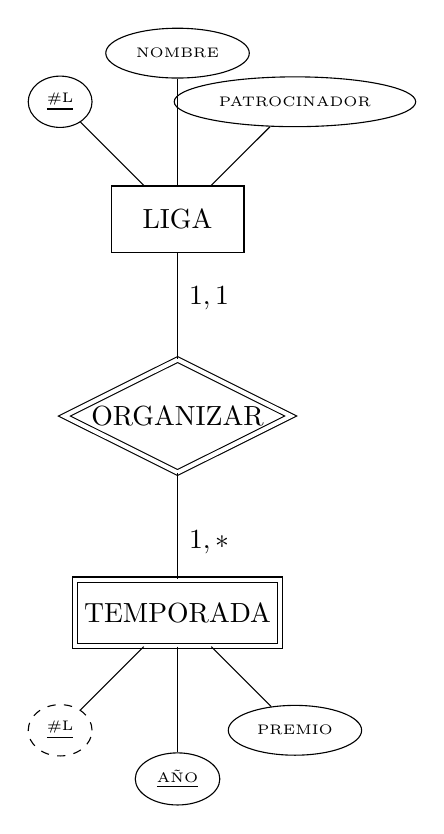
\begin{tikzpicture}[node distance=6em]
                    \node[entity] (liga) at (0,0) {LIGA}
                    [sibling distance=3cm]
                    child {node[attribute] [above of=liga] {\tiny NOMBRE}}
                    child {node[attribute] [above right of=liga] {\tiny PATROCINADOR}}
                    child {node[attribute] [above left of=liga] {\tiny \underline{\#L}} };
                    \node[entity,double distance =1.5 pt] (temp) at (0,-5) {TEMPORADA}
                    child {node[attribute,dashed] [below left of=temp] {\tiny \underline{\#L}} }
                    child {node[attribute] [below of =temp] {\underline{\tiny A\~NO}}}
                    child {node[attribute] [below right of=temp] {\tiny PREMIO}};
                  
                    \node[relationship,aspect=2,double distance =1.5 pt] (organizar) at (0,-2.5) {ORGANIZAR} edge(liga) edge(temp);

            
                    \node at (0.4,-1) {$1,1$};
                    \node at (0.4,-4.1) {$1,\ast$};
                  
                \end{tikzpicture}
                }
        \end{column}

        \begin{column}{0.48\linewidth}
            \vspace{20mm}

            \onslide<2->{

                \begin{scriptsize}
                    \textbf{Liga}(\underline{\#L}, Nombre, Patrocinador)\\[2mm]
    
                
                    \textbf{Temporada}(\underline{\#L}, \underline{A\~no}, Premio)\\[1mm]
                    \hspace{4mm} FK: \#L REFERENCES Liga
                \end{scriptsize}
            }
        \end{column}
    \end{columns}
\end{frame}


\begin{frame}{}
    \begin{columns}[T]
        \begin{column}{0.46\linewidth}
            \vspace{33mm}

            \Large \textcolor{blue3}{El dise\~no l\'ogico no es subjetivo}
        \end{column}

        \begin{column}{0.53\linewidth}
            
\includegraphics[width=\linewidth, height=0.8\textheight]{img/design.jpg}
        \end{column}
        
    \end{columns}
\end{frame}



% \begin{frame}{F\'acil}


% \end{frame}

    
\begin{frame}{Entonces...}

    \begin{columns}[T]
        \begin{column}{0.4\linewidth}
            \vspace{3.3cm}

            \Huge ... alguna duda?
        \end{column}
        \begin{column}{0.58\linewidth}
            
            
\includegraphics[height=0.8\textheight, width=\linewidth]{img/eval.jpg}
        \end{column}
        
    \end{columns}
    
\end{frame}
    \maketitle
    \begin{frame}
    \frametitle{Anexos}

    \centering
    \Huge \textcolor{blue3}{Anexos}

\end{frame}

\begin{frame}{Anexos}
    \framesubtitle{Algoritmo para determinar si un conjunto de atributos cumple la unicidad}

    \textbf{Entrada}: $U = \{A_1,A_2,...,A_n\}$, $F$ conjunto de dependencias funcionales y $X$, $X \subseteq U$\\
    \textbf{Salida}: 1 si el conjunto $X$ cumple la unicidad en $R(U,F)$ o 0 en otro caso.\\
    \textbf{M\'etodo}:
    \begin{enumerate}
        \item Sea $X$ el conjunto de atributos que se desea comprobar. Primero inicializamos
        $X_0 = X$.
        \item En cada iteraci\'on $i$ se busca una dependencia funcional $Y \to A$ tal que
        $Y \subseteq X_{i-1}$, pero $A \notin X_{i-1}$. Entonces
        se asigna $X_i = X_{i-1} \cup \{A\}$.
        \item Repetir el paso 2 tantas veces como sea necesario hasta que no puedan a\~nadirse
        m\'as atributos. Dado que el conjunto resultante solo puede crecer y la cantidad de atributos
        en el universo es finito, eventualmente el algoritmo termina.
        \item Sea $k$ la iteraci\'on final del algoritmo, se comprueba que $X_k = U$.  
        
    \end{enumerate}
\end{frame}
\end{document}
